%!TEX TS-program = xelatex
%!TEX encoding = UTF-8 Unicode
\documentclass[16pt,a4paper]{article}
\usepackage{fontspec,xltxtra,xunicode}
\usepackage[top=1.5in,bottom=1in,left=1.5in,right=1.5in]{geometry}
\usepackage{polyglossia}
\newfontfamily\thaifont{TH Sarabun New}
\setmainfont{TH Sarabun New}
\setdefaultlanguage{thai}
\XeTeXlinebreaklocale 'th'
\usepackage{scrextend}
\changefontsizes[16pt]{16pt}
\XeTeXlinebreakskip = 0pt plus 1pt
\defaultfontfeatures{Scale=1.23}
\renewcommand{\baselinestretch}{1.2}

% - - - - - - - - - - - - - - - - - - - -
% NEED BY \makethesiscover
% - - - - - - - - - - - - - - - - - - - -
\newcommand{\ThesisThaiName}{การสร้างกรณีทดสอบจากกราฟการเรียกเชิงสถิตของภาษาจาวา}
\newcommand{\ThesisEnglishName}{Test case generation from Java static call graph}
\newcommand{\studentname}{นายสิทธิพงษ์ เหล่าโก้ก}
\newcommand{\studentid}{5870972621}
\newcommand{\curriculumn}{วิทยาศาสตร์มหาบัณฑิต}
\newcommand{\major}{วิศวกรรมซอฟต์แวร์}
\newcommand{\department}{วิศวกรรมคอมพิวเตอร์}
\newcommand{\faculty}{วิศวกรรมศาสตร์}
\newcommand{\address}{17/8 หมู่ 18 ตำบลคลองหนึ่ง อำเภอคลองหลวง จังหวัดปทุมธานี 12120}
\newcommand{\telephone}{061-629-9905}
\newcommand{\emailaddress}{sitdhibong.l@student.chula.ac.th}
\newcommand{\advisor}{รองศาสตราจารย์.ดร.ธาราทิพย์ สุวรรณศาสตร์}
\newcommand{\thakeywords}{การสร้างกรณีทดสอบ, ภาษาจาวา, \scg}
\newcommand{\engkeywords}{Test case generation, Java language, Static call graph}

\newcommand{\ThesisProposalTH}{โครงร่างวิทยานิพนธ์}
\newcommand{\ThesisProposalEN}{Thesis Proposal}
\newcommand{\ThesisTopic}{หัวข้อวิทยานิพนธ์}

% - - - - - - - - - - - - - - - - - - - -
% Control words
% - - - - - - - - - - - - - - - - - - - -
\newcommand{\scg}{กราฟการเรียกเชิงสถิต}
\newcommand{\scgEN}{Static call graph}

\newcommand{\cfg}{กราฟการไหลของการควบคุม}
\newcommand{\cfgen}{Control flow graph}

\newcommand{\DDPath}{DD-Path}
\newcommand{\DDPathEN}{Decision-to-decision Path}

\newcommand{\FeasiblePath}{เส้นทางที่เป็นไปได้}
\newcommand{\FeasiblePathEN}{Feasible path}

\newcommand{\InfeasiblePath}{เส้นทางที่เป็นไปไม่ได้}
\newcommand{\InfeasiblePathEN}{Infeasible path}

\newcommand{\FeasibleAndInfeasiblePath}{เส้นทางที่เป็นไปได้และไม่ได้}
\newcommand{\FeasibleAndInfeasiblePathEN}{Feasib/Users/sitdh/Desktop/vector-Overwatch-Ana-wallpaper.jpg Infeasible path}

\newcommand{\sourcecode}{รหัสต้นฉบับ}

\newcommand{\TestDataGeneration}{การสร้างข้อมูลทดสอบ}
\newcommand{\TestDataGenerationEN}{Test data generation}

\newcommand{\RegressionTesting}{การทดสอบเชิงทดถอย}
\newcommand{\RegressionTestingEN}{Regression testing}

\newcommand{\Repository}{คลังข้อมูล}
\newcommand{\RepositoryEN}{Repository}

\newcommand{\softwareComponent}{ส่วนประกอบซอฟต์แวร์}
\newcommand{\softwareComponentEN}{Software component}

\newcommand{\IntegrationTesting}{การทดสอบผสาน}
\newcommand{\IntegrationTestingEN}{Integration testing}

\newcommand{\class}{คลาส}
\newcommand{\classEN}{Class}

\newcommand{\method}{\mbox{เมท็อด}}
\newcommand{\methodEN}{Method}

\newcommand{\attribute}{แอททริบิวต์}
\newcommand{\attributeEN}{Attribute}

\newcommand{\MethodSignature}{ลายเซ็นของเมธอด}
\newcommand{\MethodSignatureEN}{Method signature}

\newcommand{\DirectedMultiGraph}{กราฟหลายทางมีทิศทาง}
\newcommand{\DirectedMultiGraphEN}{Directed multigraph}

\newcommand{\DirectedGraph}{กราฟมีทิศทาง}
\newcommand{\DirectedGraphEN}{Directed graph}

\newcommand{\ProgramGraph}{กราฟโปรแกรม}
\newcommand{\ProgramGraphEN}{Program graph}

\newcommand{\BasisPath}{เส้นทางมูลฐาน}
\newcommand{\BasisPathEN}{ฺBasis paths}

\newcommand{\Node}{โหนด}
\newcommand{\NodeEN}{Node}

\newcommand{\Edge}{เส้นเชื่อม}
\newcommand{\EdgeEN}{Edge}

\newcommand{\PredicateNode}{{\Node}เงื่อนไขการดำเนินงาน}
\newcommand{\PredicateNodeEN}{Predicate node}

\newcommand{\TestPath}{เส้นทางทดสอบ}
\newcommand{\TestPathEN}{Test path}

\newcommand{\sourcenode}{โหนดต้นทาง}
\newcommand{\sourcenodeEN}{Source node}

\newcommand{\sinknode}{โหนดปลายทาง}
\newcommand{\sinknodeEN}{Sink node}

\newcommand{\Cyclomatic}{ความซับซ้อนไซโคลเมทิก}
\newcommand{\CyclomaticEN}{Cyclomatic Complexity}

\newcommand{\inputVector}{เวกเตอร์นำเข้า}
\newcommand{\inputVectorEN}{Input vector}

\newcommand{\CUT}{{\class}ภายใต้การทดสอบ}
\newcommand{\CUTEN}{Class under test}

\newcommand{\SUT}{ซอฟต์แวร์ภายใต้การทดสอบ}
\newcommand{\SUTEN}{Software under test}

\newcommand{\Path}{ทางเดิน}
\newcommand{\PathEN}{Path}

\newcommand{\DynamicInformation}{ข้อมูลเชิงพลวัต}
\newcommand{\DynamicInformationEN}{Dynamic information}

\newcommand{\StaticInformation}{ข้อมูลเชิงสถิต}
\newcommand{\StaticInformationEN}{Static information}

\newcommand{\testSuite}{ชุดทดสอบ}
\newcommand{\testSuiteEN}{Test suite}

\newcommand{\testCase}{กรณีทดสอบ}
\newcommand{\testCaseEN}{Test case}

\newcommand{\Package}{โปรแกรมสำเร็จ} % http://www.rirs3.royin.go.th
\newcommand{\PackageEN}{Package}

\newcommand{\expectedOutput}{ผลลัพธ์ที่คาดหวัง}
\newcommand{\expectedOutputEN}{Expected output}

\newcommand{\csp}{ปัญหาการหาค่าเหมาะที่สุดเชิงการจัด} % https://www.cp.eng.chula.ac.th/~somchai/CD/2110427/2546/demo/HW2-TSP/saTSP.htm
\newcommand{\cspEN}{Constraint satisfaction problem}

\newcommand{\Algorithm}{ขั้นตอนวิธี}
\newcommand{\AlgorithmEN}{Algorithm}

\newcommand{\software}{ซอฟต์แวร์}
\newcommand{\softwareEN}{Software}

\newcommand{\tester}{นักทดสอบซอฟต์แวร์}
\newcommand{\testerEN}{Software tester}

\newcommand{\constantExtracting}{การรวบรวมค่าคงที่}
\newcommand{\constantExtractingEN}{Constant extracting}

\newcommand{\graphCreation}{การสร้างกราฟ}
\newcommand{\graphCreationEN}{Graph creation}

\newcommand{\sourcecodeInstrumention}{แทรกคำสั่งในรหัสต้นฉบับ}
\newcommand{\sourcecodeInstrumentionEN}{Source code instrumentation}

\newcommand{\testcaseGeneration}{การสร้างกรณีทดสอบ}
\newcommand{\testcaseGenerationEN}{Test case generation}

\newcommand{\testpathSelection}{การเลือกทางเดินทดสอบ}
\newcommand{\testpathSelectionEN}{Test path selection}

\newcommand{\randomTestData}{สุ่มข้อมูลนำเข้า}
\newcommand{\randomTestDataEN}{Random test data}

\newcommand{\testData}{ข้อมูลทดสอบ}
\newcommand{\testDataEN}{Test data}

\newcommand{\testCaseGeneration}{การสร้างกรณีทดสอบ}
\newcommand{\testCaseGenerationEN}{Test case generation}

\newcommand{\expectedOutputAdjustment}{การปรับค่าคาดหวัง}
\newcommand{\expectedOutputAdjustmentEN}{Expected output adjustment}

\newcommand{\executeSoftwareTesting}{ดำเนินการทดสอบซอฟต์แวร์}
\newcommand{\executeSoftwareTestingEN}{Software testing execute}

\newcommand{\testResultCompare}{เปรียบเทียบผลลัพธ์การดำเนินงาน}
\newcommand{\testResultCompareEN}{Compare test excution result}

\newcommand{\pathConditions}{เงื่อนไขของเส้นทาง}
\newcommand{\enum}{อีนัม}

\usepackage{indentfirst}
\usepackage{graphicx}
\graphicspath{ {figures/} }
\usepackage{titlesec}
\usepackage{pdflscape}
\usepackage{tabularx}
\usepackage{mathtools}

\usepackage{algorithm} 
\usepackage{algorithmic}

\usepackage{listings}

\usepackage{rotating}
\usepackage{multirow}
\usepackage[usernames,dvipsnames,svgnames,table]{xcolor}
\definecolor{LightGray}{gray}{0.9}

\usepackage{fancyhdr}
\pagestyle{fancy}
\fancyhf{}
\rhead{\thepage}
\renewcommand{\headrulewidth}{0pt}
% \fancyhead[LO]{}
% \fancyhead[RE]{}
% \fancyfoot[C]{\thepage} 

\usepackage{subcaption}
\captionsetup[sub]{}

% - - - - - - - - - - - - - - - - - - - -
% Code listing
\usepackage{fontspec}
\setmonofont{Inconsolata}
\usepackage{verbatim}
\usepackage{lmodern}

% - - - - - - - - - - - - - - - - - - - -
% Equation
\usepackage{amsmath}

% - - - - - - - - - - - - - - - - - - - -
% Graphic
\usepackage{tikz}
\usetikzlibrary{positioning}

% - - - - - - - - - - - - - - - - - - - -
% Nested enum
\renewcommand{\labelenumii}{\theenumii}
\renewcommand{\theenumii}{\theenumi.\arabic{enumii}.}

% - - - - - - - - - - - - - - - - - - - -
% Misc config.

\titleformat{\section}{\bfseries}{\thesection}{0.4em}{}
\titleformat{\subsection}{\bfseries}{\thesubsection}{0.4em}{}
\titleformat{\subsubsection}{\bfseries}{\thesubsubsection}{0.4em}{}

\setlength\parindent{0.5in}
\setlength\parskip{.5em}
\titlespacing\section{0pt}{12pt plus 4pt minus 2pt}{0pt plus 2pt minus 2pt}
\titlespacing\subsection{0pt}{12pt plus 4pt minus 2pt}{0pt plus 2pt minus 2pt}
\titlespacing\subsubsection{0pt}{12pt plus 4pt minus 2pt}{0pt plus 2pt minus 2pt}

\lstdefinestyle{thesiscodestyle}{
    tabsize=2, numbers=left,
    breaklines=true, showspaces=false, showstringspaces=false,
    basicstyle=\listingsfont,
    language={Java},
    commentstyle=\color{eclipseGreen},
    keywordstyle=\color{eclipsePurple},
    stringstyle=\color{eclipseBlue},
}
\newfontfamily\listingsfont[Scale=.5]{Monaco} 
\newfontfamily\listingsfontinline[Scale=1.8]{Monaco} 
\definecolor{eclipseBlue}{RGB}{42,0.0,255}
\definecolor{eclipseGreen}{RGB}{63,127,95}
\definecolor{eclipsePurple}{RGB}{127,0,85}

\def\@vpt{12}

\newcommand{\FirstTimeDefine}[2]{#1\,(#2)}

\newcommand{\code}[1]{\small{$#1$}}

\newcommand{\figref}[1]{\figurename\ \ref{#1}\ }
\newcommand{\figpageref}[1]{\figurename\ \ref{#1}\ (\pagename\ \pageref{#1})\ }

\newcommand{\tabref}[1]{\tablename\ \ref{#1}\ }
\newcommand{\tabpageref}[1]{\tablename\ \ref{#1}\ (\pagename\ \pageref{#1})\ }

\newcommand{\eq}[1]{\ (\ref{#1})\ }

\newcommand{\makethesiscover}{ %

    \thispagestyle{empty}
    \begin{center}
        \bf
        {\large {\ThesisProposalTH} \\ ({\ThesisProposalEN})}
    \end{center}

    \noindent
    \begin{table}[ht!]
        \centering
        \label{tab:metadata}
        \begin{tabular*}{\linewidth}{ll@{\extracolsep{\fill}}}
            {\bf ชื่อเรื่อง (ภาษาไทย)}      & \ifdefined\ThesisThaiName \ThesisThaiName\fi          \\
            {\bf ชื่อเรื่อง (ภาษาอังกฤษ)}    & \ifdefined\ThesisEnglishName \ThesisEnglishName\fi    \\ \\
            {\bf เสนอโดย}               & \ifdefined\studentname \studentname\fi                \\
            {\bf รหัสนิสิต}                & \ifdefined\studentid \studentid\fi                    \\
            {\bf หลักสูตร}                & \ifdefined\curriculumn \curriculumn\fi                \\
            {\bf สาขา}                  & \ifdefined\major \major\fi                            \\
            {\bf ภาควิชา}                & \ifdefined\department \department\fi                  \\
            {\bf คณะ}                   & \ifdefined\faculty \faculty\fi                        \\
            {\bf สถานที่ติดต่อ}             & \ifdefined\address \address\fi                        \\
            {\bf โทรศัพท์}                & \ifdefined\telephone \telephone\fi                    \\
            {\bf อีเมล}                  & \ifdefined\emailaddress \emailaddress\fi              \\
            {\bf อาจารย์ที่ปรึกษา}          & \ifdefined\advisor \advisor\fi                        \\ \\
            {\bf คำสำคัญภาษาไทย}         & \ifdefined\thakeywords \thakeywords\fi                \\
            {\bf คำสำคัญภาษาอังกฤษ}       & \ifdefined\engkeywords \engkeywords\fi                \\
        \end{tabular*}
    \end{table}

    \clearpage
}

\newcommand{\ThesisTitlePage}{
    \begin{center}
        {\bf\large {\ThesisProposalTH}}
    \end{center}

    {\noindent\bf \ThesisTopic}

    \begin{table}[ht!]
        \centering
        \label{tab:thesisname}
        \begin{tabular*}{\linewidth}{ll@{\extracolsep{\fill}}}
            {\bf ภาษาอังกฤษ} & {\ifdefined\ThesisEnglishName \ThesisEnglishName\fi} \\
            {\bf ภาษาไทย}   & {\ifdefined\ThesisThaiName \ThesisThaiName \fi} \\
        \end{tabular*}
    \end{table}
    
}


\begin{document}

    \pagenumbering{alphabet}

\begin{table}[ht!]
    \center
    \begin{tabularx}{\textwidth}{|l|l|X|}
        \hline
        \rowcolor{LightGray}
        {\bf วันที่}   & {\bf จุดแก้ไข}          & {\bf บันทึกการแก้ไข} \\ \hline
        2 ธันวาคม    & สถิต หรือ สถิตย์          & ตรวจสอบจากพจานานุกรมฉบับสำนักงานราชบัณฑิตยสภาเรียบร้อยแล้ว \\ \hline
%                                                ใช้คำว่า {\it "สถิต"} ส่วนคำว่า {\it "สถิตย์"} ไม่มีในพจนานุกรมครับ \\ \hline
%                    & รูปที่ x (หน้า n)         & ตัดคำว่า\ {\bf (หน้า n)}\ ทิ้งไป \\ \hline
    \end{tabularx}
\end{table}

    \clearpage

    \makethesiscover

    \pagenumbering{arabic}
    \ThesisTitlePage

    \section{ที่มาและความสำคัญ} 
\label{sec:introduction}

การทดสอบซอฟต์แวร์เป็นขั้นตอนที่ทำขึ้นเพื่อค้นหาข้อผิดพลาดที่ยังคงอยู่ภายในซอฟต์แวร์ \cite{Myers:2011:AST:983238}
อีกทั้งยังเป็นกระบวนการสร้างความมั่นใจด้านคุณภาพของซอฟต์แวร์ที่ได้พัฒนาขึ้น ดังนั้นกว่ากึ่งหนึ่งของทรัพยากรที่ใช้ในการดำเนินงานโครงการพัฒนาซอฟต์แวร์
จึงถูกจัดสรรค์ให้กับขั้นตอนการทดสอบซอฟต์แวร์นี้ \cite{Jackson2007, Tassey2002} ดังนั้นการทดสอบซอฟต์แวร์จึงถือเป็นขั้นตอนที่สำคัญ
ในกระบวนการพัฒนาซอฟต์แวร์อีกขั้นตอนหนึ่ง

การพัฒนาซอฟต์แวร์นั้นมีแนวทางการพัฒนาหลากหลายแนวทางด้วยกัน ไม่ว่าจะเป็นการกำหนดแนวทางการพัฒนาด้วยการทดสอบ (Test-Driven Development) 
ที่จะสร้างกรณีทดสอบย่อย (Unit Testing) เพื่อกำหนดพฤติกรรมการทำงานของคลาสที่สนใจหรือคลาสภายใต้การทดสอบ (Class under test) 
ก่อนที่จะเริ่มพัฒนาซอฟต์แวร์จริง \cite{Markovi2012} และการพัฒนาโดยใช้พฤติกรรมการใช้งาน (Behaviour-Driven Development) 
ซึ่งกำหนดลักษณะการใช้งานซอฟต์แวร์แล้ว จึงพัฒนาส่วนประกอบของซอฟต์แวร์ที่สอดคล้องกับการใช้งานนั้น \cite{Lazar2010}
ซึ่งทั้ง 2 แนวทางนั้นจะสร้างกรณีทดสอบ เพื่อใช้ในการทดสอบส่วนย่อย (Unit Testing) โดยจะจำลองพฤติกรรมการทำงานของคลาสหรือส่วนประกอบอื่น ๆ
(Mocking) เช่น ฐานข้อมูล เว็บเซอร์วิส หรืออุปกรณ์เชื่อมต่อที่ต้องการ ที่มีปฏิสัมพันธ์กับคลาสภายใต้การทดสอบ ในลักษณะของ (Stub) และไดรเวอร์ (Driver)
เพื่อจำกัดขอบเขตของข้อผิดพลาดให้อยู่เฉพาะแต่เพียงคลาสภายใต้การทดสอบเท่านั้น แต่เพื่อให้มั่นใจได้ว่าซอฟต์แวร์สามารถทำงานร่วมกันได้ 
ตามพฤติกรรมที่ได้จำลองไว้สตับและไดรเวอร์ในขั้นตอนการการทดสอบย่อยนั้น 
จึงจำเป็นจะต้องทดสอบการทำงานร่วมกันด้วย\FirstTimeDefine{\IntegrationTesting}{\IntegrationTestingEN}
โดยในขั้นตอนนี้ จะใช้การเชื่อมต่อไปยังส่วนประกอบที่มีปฏิสัมพันธ์กับกระบวนการนั้นโดยตรง เพื่อให้มั่นใจได้ว่าซอฟต์แวร์ภายใต้การทดสอบ (Software under test) 
สามารถดำเนินงานตามกระบวนการที่สนใจได้โดยไม่เกิดข้อขัดข้อง

ทั้งนี้ การสร้างกรณีทดสอบในขั้นตอนก{\IntegrationTesting}นั้นจะสร้างกรณีทดสอบสอดคล้องตามกระบวนการทำงานของ\FirstTimeDefine{\SUT}{\SUTEN} 
โดยผลลัพธ์ที่เป็นไปได้ย่อมเกิดระหว่างการเรียกใช้งานระหว่าง{\softwareComponent}ภายใน{\SUT}ด้วยกันเอง ตลอดจนส่วนประกอบภายนอก 
ซึ่งล้วนแล้วแต่มีหลายปัจจัยที่ต้องนำมาพิจารณาร่วมกัน การสร้างกรณีทดสอบอัตโนมัติจึงมีบทบาทสำคัญ สำหรับช่วยให้การสร้างกรณีทดสอบทำได้รวดเร็วมากยิ่งขึ้น 
หากแต่การสร้างกรณีทดสอบในขั้นตอน{\IntegrationTesting} ยังต้องใช้\FirstTimeDefine{\DynamicInformation}{\DynamicInformationEN}
ได้จากการสั่งกระทำการ (Execute) ระหว่างชุดกรณีทดสอบกับ{\sourcecode} โดยข้อมูลที่ได้จากวิธีการนี้สามารถอธิบายพฤติกรรมของ{\SUT}ของ{\sourcecode}
ได้เป็นอย่างดี หากแต่การเปลี่ยนแปลงของ{\sourcecode}นั้นอากเกิดขึ้นภายหลังจากที่ได้สั่งกระทำการชุดทดสอบไปแล้ว 
ส่งผลให้ชุดทดสอบนั้นไม่สามารถอธิบายคุณลักษณะของ{\sourcecode}ที่เป็นปัจจุบันได้ ดังนั้นหากสามารถนำ\FirstTimeDefine{\StaticInformation}{\StaticInformationEN}
ที่ได้จาก{\sourcecode}ที่เป็นปัจจุบัน มาใช้เป็นข้อมูลในขั้นตอนการสร้างชุดทดสอบให้ครอบคลุมตามความสัมพันธ์ระหว่าง{\softwareComponent}ซึ่งปรากฎใน{\SUT} 
จะทำให้ชุดทดสอบนั้น สามารถอธิบายคุณลักษณะตลอดจนการดำเนินงานของ{\SUT}ที่เป็นปัจจุบันได้

ดังนั้น การวิจัยนี้จึงต้องการที่จะนำเสนอแนวทางการสร้างกรณีทดสอบ บน{\TestPath}ซึ่งพิจารณาจากความสัมพันธ์ระหว่าง{\softwareComponent} 
ที่ด้วยรวบรวมได้จากข้อมูล{\StaticInformation}ของ{\sourcode}ภายใน{\Package}ภายใน{\SUT} พร้อมด้วยการสร้างข้อมูลทดสอบ (Test data) 
ที่สอดคล้องตามเงื่อนไขที่ปรากฏอยู่บน{\TestPath} ที่เลือก ทั้งนี้เพื่อให้ชุดทดสอบที่สร้างขึ้นสามารถทดสอบแต่ละ{\Path}ระหว่าง{\softwareComponent}อย่างน้อย 1 ครั้ง
โดยใช้ผลลัพธ์ที่เกิดจากการสั่งกระทำการชุดกรณีทดสอบที่สร้างขึ้นกับ{\sourcecode}ซึ่งผ่านการแทรกชุดคำสั่งสำหรับติดตามการทำงาน 
เพื่อตรวจสอบว่า กรณีทดสอบนั้นสามารถทดสอบทุกความสัมพันธ์ระหว่าง{\softwareComponent}ได้ตามที่ต้องการ


    \section{ทฤษฎีที่เกี่ยวข้อง} 

% ต้องปรับเพิ่ม
เพื่อให้ทราบถึงแนวทางการวิจัยที่สามารถทำได้ จึงจำเป็นจะต้องศึกษาวิธีการ หรือทฤษฎีต่างๆ ซึ่งน่าจะเป็นประโยชน์ต่อการดำเนินการวิจัย
ให้สามารถดำเนินได้อย่างลุล่วงไว้ดังนี้

\subsection{\FirstTimeDefine{\ProgramGraph}{\ProgramGraphEN}} 
\label{sec:sub:pg}

{\software} ถูกพัฒนาขึ้นมาเพื่อแก้ไขปัญหาในบริบทที่หลากหลาย ส่งผลให้มีโครงสร้างของ{\sourcecode}นั้นแตกต่างกันไปตามบริบทการพัฒนา
หรือปัญหาที่ต้องการแก้ไข ซึ่งไม่มีรูปแบบโครงสร้างที่คงตัว หากแต่ในขั้นตอนสร้างกรณีทดสอบนั้น\FirstTimeDefine{\tester}{\testerEN}
จำเป็นต้องทำความเข้าใจโครงสร้างของ{\software} ทั้งจากแผนภาพการออกแบบ เช่น แผนภาพยูเอ็มแอล (UML - Unified Modeling Language) 
และจาก{\sourcecode}โดยตรง ซึ่งการทำความเข้าใจโครงสร้างผ่าน{\sourcecode}โดยตรงนั้นย่อมสะท้อนลักษณะของ{\software}ที่เป็นปัจจุบันมากที่สุด
{\ProgramGraph} จึงเป็นวิธีการนำเสนอโครงสร้างที่ปรากฏอยู่ภายใน{\software} ณ ขณะที่สนใจ ช่วยให้{\tester}เข้าใจโครงสร้างของ{\software}
และออกแบบกรณีทดสอบได้มีประสิทธิภาพมากยิ่งขึ้น ซึ่งในงานวิจัยนี้จะนำ{\ProgramGraph}มาใช้ 2 ประเภท ด้วยกัน ได้แก่

\subsubsection{\FirstTimeDefine{\cfg}{\cfgen}}
\label{sec:sub:sub:cfg}

หากแทน{\software} \code{P} แทนด้วยกราฟ \code{G} จะได้ว่า \code{G = (V, A)} เมื่อ \code{V (Vertex)} 
คือเซตของ{\Node}ในกราฟ ซึ่งแต่ละ{\Node}แทนแถวคำสั่งใน{\sourcecode} และ \code{A\ (Arcs)} 
คือเซตของคู่ลำดับโหนดที่มีความสัมพันธ์กันภายในกราฟซึ่งเชื่อมต่อกันแบบมีทิศทาง หาก \code{(v_m, v_n) \in A} จะหมายถึง 
"\Node\ \code{v_n} จะทำงานในลำดับถัดไปหลังจากที่ \code{v_m} ทำงานเสร็จสิ้น" \cite{Jorgensen2013} 
โดยที่ \code{v_i, v_j \in V} มีโหนดซึ่งไม่มีดีกรีเข้า \code{(d^+(v_i) = 0)} เป็นโหนดเริ่มต้น (Source node) 
และโหนดซึ่งไม่มีดีกรีออก \code{(d^-(v_j) = 0)} เป็นโหนดปลาย (Sink node) 
กล่าวได้ว่า{\cfg}นั้นถือว่าเป็นกราฟอวัฏจักรระบุทิศทาง (Directed acyclic graph: DAG) \cite{Bang-Jensen2009}\ 
ซึ่งรูปแบบความสำพันธ์ของกราฟโปรแกรมนั้น McCabe \cite{Watson1996} 
ได้เสนอรูปแบบโครงสร้างการทำงานขั้นพื้นฐานของการพัฒนาโปรแกรม (The primitive operations of structured programming) 
\figref{fig:graphtype}

\begin{figure}[ht!]
    \centering
    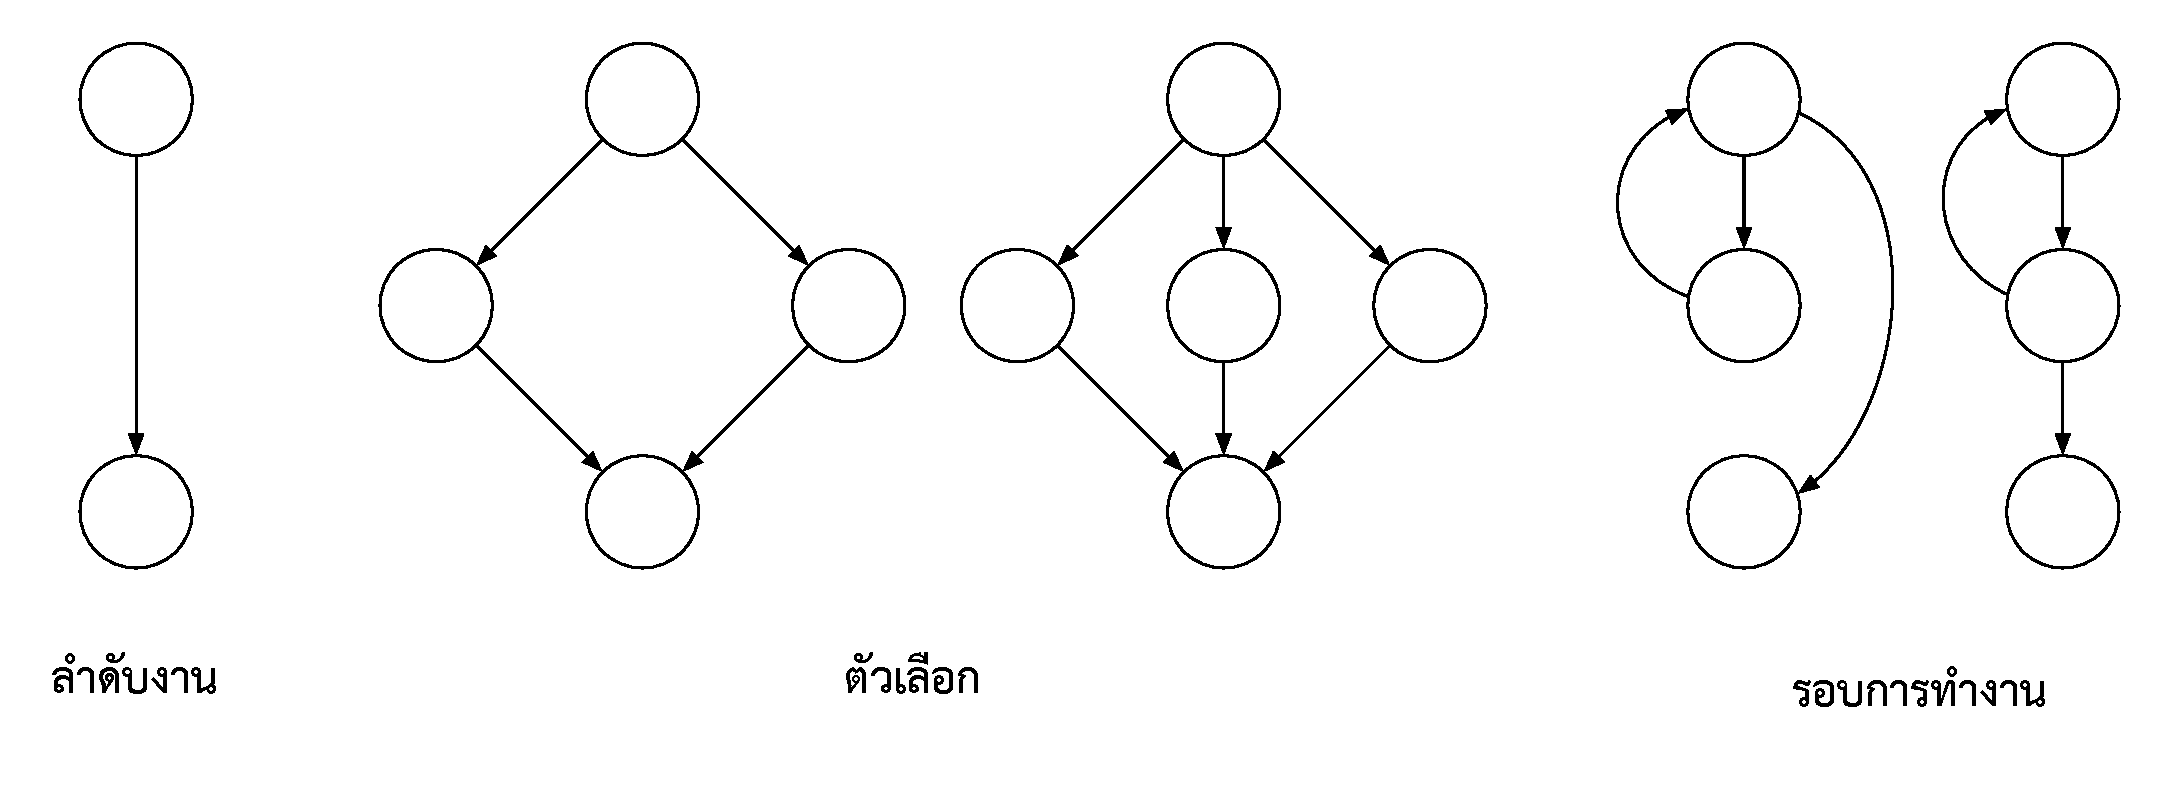
\includegraphics[width=0.9\textwidth]{graph-types}
    \caption{ประเภทของกราฟ}
    \label{fig:graphtype}
\end{figure}

จาก\figref{fig:pseudocodeGrading} เป็นรหัสเทียม (Psuedo code) ที่นำเสนอวิธีการคำนวณเกรดของนิสิตโดยรับข้อมูลคะแนน \code{(student\_score)} 
และคะแนนพิเศษ \code{(bonus\_score)} ของนิสิต หากมีคะแนนเป็น 0 จะได้เกรด \code{I}\ หากนิสิตได้คะแนนต่ำกว่า 80 คะแนน 
จะได้เกรด \code{U}\ หากมีคะแนนตั้งแต่ 80 ไปจนถึง 100 คะแนน นิสิตจะได้เกรด \code{S}\ ซึ่งจากชุดรหัสเทียมนี้ 
สามารถแปลงเป็นกราฟโปรแกรม เพื่อทำความเข้าใจโครงสร้างได้ดัง{\figref{fig:programGraph} 

\begin{figure}[ht!]
    \begin{algorithm}[H]
        \begin{algorithmic}[1]
            \STATE{Program {\bf "Simple Grading"}}
            \STATE{student\_score $\gets$ receive student score}
            \STATE{bonus\_score $\gets$ receive student's bonus score}

            \IF{bonus\_score > 0}
                \IF{student\_score <= 50} 
                    \STATE{student\_score = min(50, student\_score + bonus\_score)} 
                \ELSIF{student\_score <= 70} 
                    \STATE{student\_score = min(70, student\_score + bonus\_score)}
                \ENDIF
            \ENDIF

            \STATE{grade\_letter = ""}

            \IF{student\_score < 80} 
                \STATE{grade\_letter = 'U'} 
            \ELSIF{student\_score == 0}
                \STATE{grade\_letter = 'I'} 
            \ELSIF{student\_score <= 100}
                \STATE{grade\_letter = 'S'} 
            \ENDIF

            \STATE{print(grade\_letter)}
        \end{algorithmic}
    \end{algorithm}
    \caption{ชุดรหัสเทียมสำหรับคำนวณเกรดนิสิตจากคะแนนที่ได้รับ}
    \label{fig:pseudocodeGrading}
\end{figure}


\begin{figure}[ht!]
    \centering
    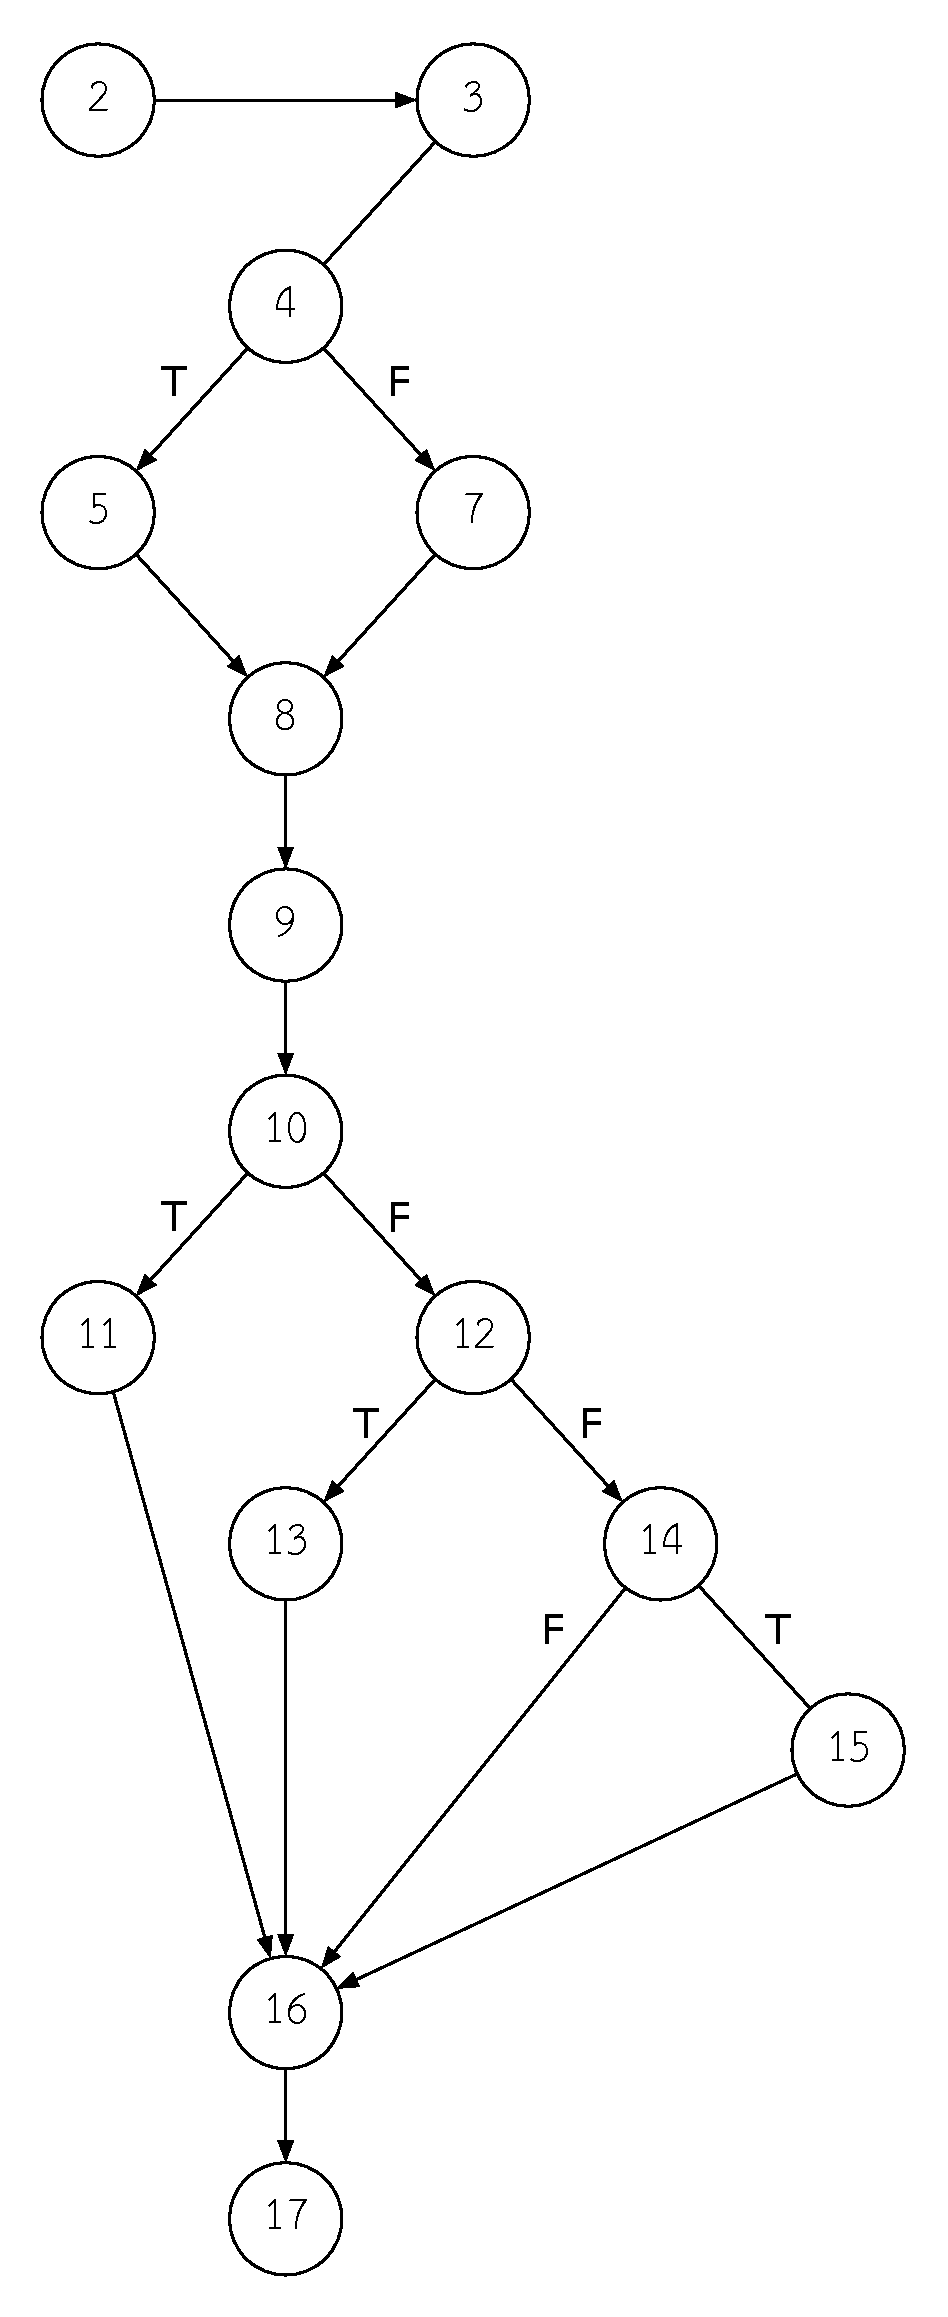
\includegraphics[height=0.80\textheight]{grading-program-graph}
    \caption{{\cfg}ของชุดรหัสเทียมสำหรับคำนวณเกรดนิสิต}
    \label{fig:programGraph}
\end{figure}

จาก{\figref{fig:programGraph}} เป็นการนำเสนอชุดรหัสเทียมจาก{\figref{fig:pseudocodeGrading} ในรูปของกราฟโปรแกรม 
โดยที่{\Node}ที่ 2, 3, 6, 8, 9, 10, 11, 13, 17, 18 และ 19 คือ{\Node}ที่แสดงถึงลำดับการดำเนินงาน 
และ{\Node} 4, 5, 6, 7, 12, 14 และ 16 เป็น{\FirstTimeDefine{\PredicateNode}{\PredicateNodeEN}} ภายในโปรแกรม 
โดยมีโหนด 2 และ 19 เป็น{\sourcenode} และ{\sinknode} ตามลำดับ 

จากโครงสร้าง{\sourcecode} ดัง{\figref{fig:pseudocodeGrading}} ทำให้เห็นได้ว่า {\tester}สามารถทำความเข้าใจโครงสร้างของ{\sourcecode} ได้ 
ถึงแม้{\tester}จะไม่มีประสบการณ์กับภาษาที่ใช้พัฒนา หากแต่{\tester}สามารวิเคราะห์หากรณีทดสอบได้จาก{\cfg}ข้างต้น 
ด้วยการพิจารณา{\PredicateNode}ที่ปรากฏบน{\FirstTimeDefine{\TestPath}{\TestPathEN}} ยกตัวอย่างเช่น 
หากเลือก{\Path}จาก{\figref{fig:programGraph}} เป็น{\TestPath}ดังที่แสดงใน{\figref{fig:testpath}} จะพบว่ามี{\PredicateNode}บน{\TestPath} 3 {\Node} 
ด้วยกัน นั่นคือ \code{4}, \code{5} และ \code{10} เมื่อพิจารณา{\PredicateNode}ทั้ง 3 {\Node}จะได้ข้อมูลทดสอบเป็น \code{bonus\_score = 1} และ 
\code{student\_score = 50} ซึ่งข้อมูลทดสอบที่สร้างขึ้นนี้สามารถทำให้โปรแกรมทำงานใน{\TestPath}ได้ 
ดังกรณีทดสอบใน\tabref{tab:simpleTestCase}

\clearpage
\begin{figure}[ht!]
    \centering
    \code{2\ - 3\ - (4)\ - (5)\ - 6\ - 10\ - 11\ - (12)\ - 13\ - 18 - 19}
    \caption{ตัวอย่าง{\TestPath}สำหรับโปรแกรมคำนวณเกรด}
    \label{fig:testpath}
\end{figure}


\begin{table}[ht!]
    \centering
    \caption{กรณีทดสอบ}
    \label{tab:simpleTestCase}
    \begin{tabular}{|l|c|c|c|}
        \hline
        \rowcolor{LightGray}
        Case ID     & bonus\_score  & student\_score    & Expected output \\
        \hline
        SC1         & 1             & 50                & U \\
        \hline
    \end{tabular}
\end{table}

\subsubsection{\FirstTimeDefine{\scg}{\scgEN}}

การพัฒนา{\software}เชิงวัตุ (Object-oriented programming: OOP) เป็นการรวมพฤติกรรมและความสามารถที่คล้ายคลึงกันเข้าไว้ด้วยกัน \cite{kindler2011}
ในลักษณะของ\FirstTimeDefine{\class}{\classEN} \FirstTimeDefine{\method}{\methodEN} และ \FirstTimeDefine{\attribute}{\attributeEN} 
ดังนั้นหากต้องทำเข้าใจถึงการมีปฏิสัมพันธ์ระหว่าง{\class}ภายในซอฟต์แวร์ภายใต้การทดสอบ (Software under test: SUT) จาก{\sourcecode} 
ที่ได้รับมานั้น{\scg}จึงเข้าช่วยแสดงความสัมพันธ์ในรูปแบบของ\FirstTimeDefine{\DirectedMultiGraph}{\DirectedMultiGraphEN}\ หากให้แทน{\software} \code{P} 
แทนด้วยกราฟ \code{G} จึงสามารถเขียนความสัมพันธ์ในรูปของทูเปิ้ล 6 รายการ \code{G = (V, E, tail, head, \ell_V, \ell_E, \sigma, \delta)}

\begin{table}[ht!]
    \begin{tabular}{ll}
        เมื่อ & \code{V} คือ เซตซึ่งมีสมาชิกจำกัดซึ่งเป็น{\Node}ภายในกราฟ \\
            & \code{E} คือ เซตซึ่งมีสมาชิกจำกัดของ{\Edge} \\
            & \code{tail:E \rightarrow V} คือ ฟังก์ชันซึ่งกำหนด{\Edge}ให้กับ{\Node}หาง (tail) \\
            & \code{head:E \rightarrow V} คือ ฟังก์ชันซึ่งกำหนด{\Edge}ให้กับ{\Node}หัว (head) \\
            & \code{\ell_V:V \rightarrow tail} คือ ฟังก์ชันที่กำหนดแผ่นป้ายให้กับ{\Node} \\
            & \code{\ell_E:E \rightarrow head} คือ ฟังก์ชันที่กำหนดแผ่นป้ายให้กับ{\Edge} \\
    \end{tabular}
\end{table}

\begin{figure}[htb!]
    \lstset{basicstyle=\small,style=thesiscodestyle,language=java}
    \lstinputlisting[language=Java]{related/SimpleQuiz.java}
    \caption{{\sourcecode}ภาษาจาวาสำหรับอ่านคะแนนคำถามภายในชั้นเรียน}
    \label{fig:javaQuiz}
\end{figure}

\begin{figure}[htb!]
    \lstset{basicstyle=\small,style=thesiscodestyle,language=java}
    \lstinputlisting[language=Java]{related/SimpleBonusScore.java}
    \caption{{\sourcecode}ภาษาจาวาสำหรับคำนวนคะแนนเพิ่มพิเศษ}
    \label{fig:javaBonusScore}
\end{figure}

\begin{figure}[htb!]
    \lstset{basicstyle=\small,style=thesiscodestyle}
    \lstinputlisting[language=Java]{related/SimpleGrading.java}
    \caption{{\sourcecode}ภาษาจาวาสำหรับคำนวณเกรดนิสิต}
    \label{fig:javaGrading}
\end{figure}

หาก{\class} \code{SimpleQuiz}, \code{SimpleBonusScore} และ \code{SimpleGrading} ดังแสดงใน 
\figref{fig:javaQuiz}, \ref{fig:javaBonusScore} และ \ref{fig:javaGrading} แทนด้วย \code{Q}, \code{B} และ \code{G} ตามลำดับ
จะสามารถสร้าง{\scg}เพื่ออธิบายความสัมพันธ์ของ{\class}ทั้ง 3 นี้ได้ดัง \figref{fig:scggrading} 
โดยมี{\method}ต้นทางที่เรียกใช้งานและ{\method}ปลายทางที่ถูกเรียกใช้ เป็นป้ายกำกับ

\clearpage
\begin{figure}[htb!]
    \centering
    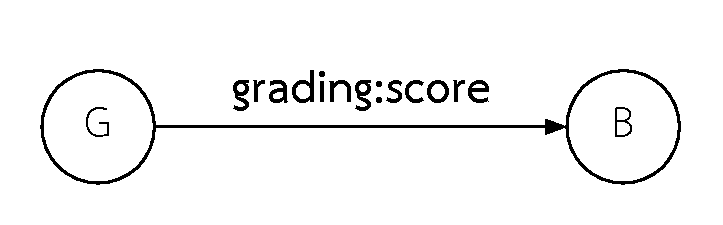
\includegraphics[width=0.8\textwidth]{simple-static-call-graph}
    \caption{{\scg}โปรแกรมคำนวณเกรดนิสิต}
    \label{fig:scggrading}
\end{figure}

% - - - - - - - - - - - - - - - - - - - -
\subsection{\FirstTimeDefine{\InfeasiblePath}{\InfeasiblePathEN}}
\label{sec:sub:infeasible-path}

\InfeasiblePath คือ ทางเดินที่ไม่สามารถหาค่าทุก ๆ ความเป็นไปได้ซึ่งสอดคล้องกับ{\PredicateNode}ที่อยู่บนทางเดินนั้น 
เพื่อทำให้โปรแกรมทำงานบนเส้นทางนั้นได้ \cite{Naik2008} หากพิจารณาจากชุดรหัสเทียมใน{\figref{fig:pseudocodeGrading}} 
และกราฟใน\figref{fig:programGraph} ประกอบเข้าด้วยกัน จะพบว่าทางเดิน 
\code{\overline{12}\ - 14\ - 15 - 18 - 19} คือ {\bf \InfeasiblePath} 
ดังแสดงใน{\figref{fig:infeasiblePath}} เนื่องจากไม่สามารถหาค่าที่สอดคล้อง กับ\PredicateNode\ 12 และ 14 
นั่นคือ \code{student\_score \geq 80} และ \code{student\_score = 0} ได้ในทุก ๆ กรณี

\begin{figure}[hbt!]
    \centering
    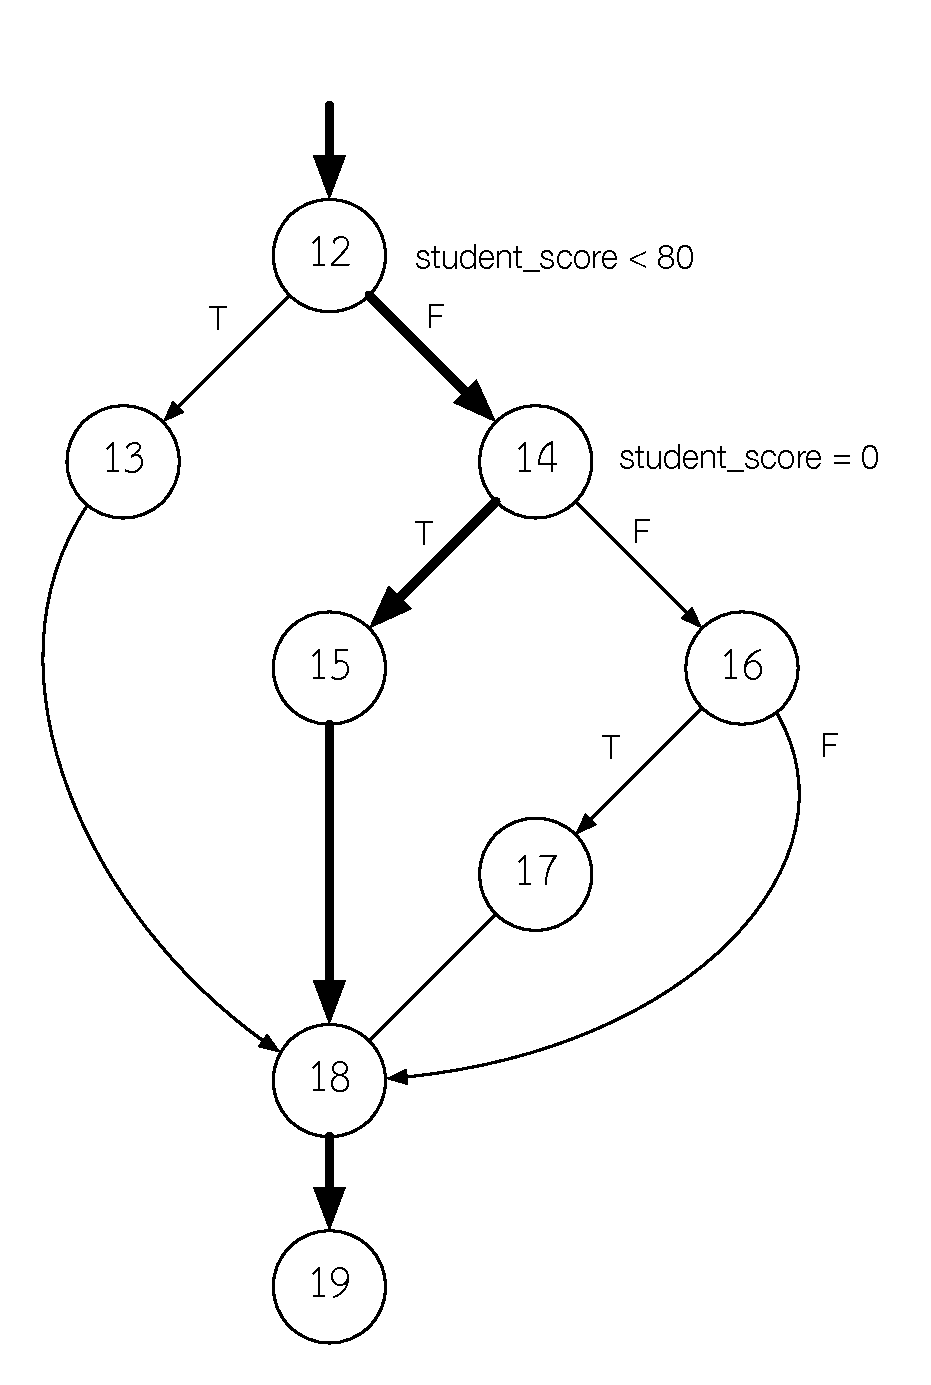
\includegraphics[width=0.4\textwidth]{grading-subgraph-infeasible-path}
    \caption{โครงสร้างของโปรแกรมที่พบ{\InfeasiblePath}}
    \label{fig:infeasiblePath}
\end{figure}


ดังนั้นการทดสอบโปรแกรมนั้นจึงจำเป็นจะต้องวิเคราะห์{\InfeasiblePath}ที่อยู่ภายในโครงสร้างของโปรแกรมเพื่อรายงานผลให้นักพัฒนาได้ทราบและแก้ไข
ต่อไปได้

\clearpage


\subsection{การสร้างกรณีทดสอบอัตโนมัติ (Automated test case generation)}

% - อ้างอิงจาก "An orchestrated survey of methodologies for automated software test case generation" \cite{Anand2013} Part II
กระบวนการทดสอบซอฟต์แวร์นั้นสามารถสร้างกรณีทดสอบอัตโนมัติ ซึ่ง Anand และคณะ \cite{Anand2013} ได้แบ่งวิธีการสร้างกรณีทดสอบแบบอัตโนมัติไว้
4 กลุ่มวิธีการด้วยกัน ได้แก่ 

\subsubsection{Symbolic execution}

วิธีการนี้เป็นกระบวนการสร้างกรณีทดสอบที่ใช้การวิเคราะห์ชุดคำสั่งควบคุมการไหลของโปรแกรมแล้วสร้างเป็นเงื่อนไขของทางเดิน (Path constraint: PC) 
เพื่อใช้วิเคราะห์หาข้อมูลที่สามารถทำให้กรณีทดสอบนั้นสามารถทดสอบทางเดินที่เลือกได้ ซึ่งวิธีนี้มีประสิทธิผลเรื่องความครอบคลุมของ{\sourcecode}ได้เป็นอย่างดี
หากแต่มีข้อเสียที่พบคือ โปรแกรมที่ใช้งานจริงนั้นมักจะมีเงื่อนไขหลากหลายและซับซ้อนเกินกว่าจะสร้างข้อมูลทดสอบอย่างอัตโนมัติได้ทั้งหมด 
นอกจากนั้นยังจำเป็นจะต้องอาศัยการตัดสินใจจากผู้ใช้งานในบางกรณี

% วิธีการที่ใช้แก้ปัญหาของ Symbolic Execution

\subsubsection{Model-based testing}

ขั้นตอนการทดสอบด้วย Model-based นั้นจะเริ่มต้นด้วยการจำลองพฤติกรรมของโปรแกรมที่ต้องการทดสอบออกมาเป็นรูปแบบการตัดสินใจ หรือแบบจำลองทางคณิตศาสตร์
ได้แก่ $p(x) \rightarrow f(g(x), a) = h(x)$ เมื่อ $f$, $g$ และ $h$ เป็นลักษณะการทำงานที่ทำให้โปรแกรมทำงานตามเงื่อนไข $p$ ที่กำหนด 
ด้วยข้อมูล $x$ ที่ป้อนให้กับโปรแกรม ทำให้เริ่มต้นการทดสอบได้โดยไม่มี{\sourcecode} แต่ปัญหาของวิธีนี้คือไม่สามารถทดสอบได้ครอบคลุมทุกกรณีและสภาพแวดล้อม

\subsubsection{Combinatorial testing}

วิธีการนี้เป็นวิธีการพื้นฐานของการทดสอบซอฟต์แวร์ เน้นไปยังการเลือกข้อมูลนำเข้าที่ทำให้ครอบคลุมส่วนของโปรแกรมที่ต้องการทดสอบ โดยกระบวนการทดสอบนั้น
เริ่มต้นด้วยการกำหนดปัจจัยที่จะทดสอบ ($f_i$) จากนั้นจึงกำหนดค่าที่เป็นไปได้ทั้งหมดของปัจจัยนั้นที่ครอบคลุมกับส่วนที่ต้องการทดสอบทั้งหมด 
(${x_1, x_2, x_3, ..., x_j}$) กรณีทดสอบที่เป็นไปได้จึงสามารถคำนวณได้จากผลคูณคาร์ทีเซียน (Cartisian product) ของจำนวนปัจจัยที่พิจารณา 
และจำนวนของค่าของที่ใช้ทดสอบสำหรับแต่ละปัจจัยนั้น เช่น หากมีปัจจัยที่ต้องพิจารณาทั้งสิ้น 4 ปัจจัย โดยที่แต่ละปัจจัยนั้นมีค่าที่เป็นไปได้ 5 ค่า ดังนั้น 
จะมีจำนวนกรณีทดสอบที่ต้องสร้างขึ้นจำนวน $4^5$ หรือ 1024 กรณี ที่ต้องจัดเตรียม จะเห็นได้ว่าวิธีการนี้มีกรณีทดสอบที่ต้องจัดเตรียมมาก 
อีกทั้งการเลือกค่าที่จะนำมาใช้ทดสอบของแต่ละปัจจัยนั้นจำเป็นจะต้องใช้ความชำนาญของผู้ทดสอบเป็นสำคัญ

\clearpage
\subsubsection{Random testing}

จากศึกษาพบว่าข้อมูลที่ทำให้เกิดข้อผิดพลาดนั้นมีแนวโน้มที่จะอยู่รวมกันเป็นรูปแบบ %ดัง{\figpageref{fig:failureRegionPattern}} 
ดังนั้น กรณีทดสอบที่สร้างขึ้น
ควรจะต้องกระจายให้ครอบคลุมทั้งกลุ่มข้อมูลนำเข้า (Input domain) เพิ่มโอกาสการค้นหาข้อผิดพลาดภายในโปรแกรม ซึ่งมีแนวทาง Adaptive Random Testing
โดย Chan และคณะ \cite{Chan2004}\ ที่พัฒนาขึ้นเพื่อเพิ่มประสิทธิภาพของ Random testing ในรูปแบบเดิม แต่ปัญหาของการทำ Random testing
นั้นก็เกิดมาจากการต้องการสุ่มค่านั้นเอง เพราะมีโอกาสที่ค่าที่สุ่มขึ้นมานั้นมีจำนวนมาและไม่สามารถค้นพบข้อผิดพลาดที่อยู่ภายในโปรแกรมเลย 
ดังนั้นวิธีการหนึ่งที่มักจะอ้างถึงใน Adaptive Random Testing นั้นก็คือการกำหนดกลุ่มข้อมูลที่เป็นไปได้ (Fixed-Sized-Candidate-Set: FSCS-ART) 
ของ Adaptive Random Testing ด้วยการกำหนดค่าสูงสุดหรือต่ำสุดที่ต้องการสุ่มค่าออกมากได้ กำหนดรูปแบบหรือประเภทของข้อมูลที่ต้องการสุ่ม 
เพื่อให้ค่าที่สุ่มขึ้นมานั้นมีโอกาสในการค้นพบข้อผิดพลาดมากขึ้น % ใกล้เคียงกับความต้องการมากที่สุด

% \begin{figure}[ht!]
%     \begin{minipage}[t]{0.3\linewidth}
%         \centering
%         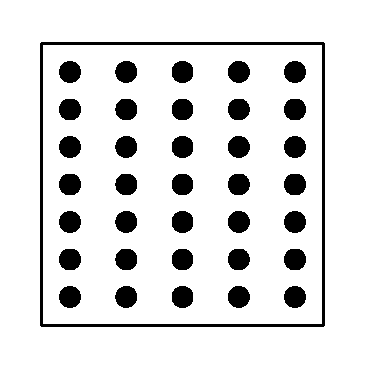
\includegraphics[width=0.6\textwidth]{failure-region-dots}
%         \subcaption{รูปแบบจุด (Dot pattern)}
%         \label{fig:subFailureDotPattern}
%     \end{minipage}
%     \begin{minipage}[t]{0.3\linewidth}
%         \centering
%         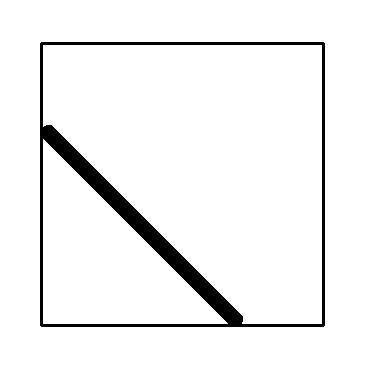
\includegraphics[width=0.6\textwidth]{failure-region-line}
%         \subcaption{รูปแบบเส้น (Strip pattern)}
%         \label{fig:subFailureStripPattern}
%     \end{minipage}
%     \begin{minipage}[t]{0.3\linewidth}
%         \centering
%         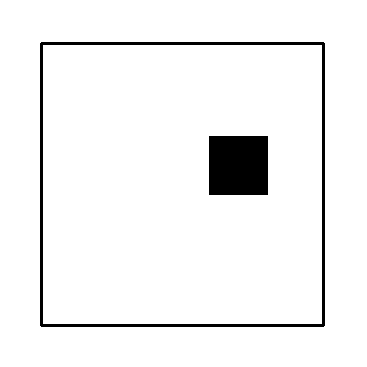
\includegraphics[width=0.6\textwidth]{failure-region-box}
%         \subcaption{รูปแบบกล่อง (Box pattern)}
%         \label{fig:subFailureBoxPattern}
%     \end{minipage}
%     \caption{รูปแบบข้อผิดพลาด \cite{Chan2004}}
%     \label{fig:failureRegionPattern}
% \end{figure}


% \subsection{\FirstTimeDefine{\inputVector}{\inputVectorEN}}


\subsection{การสร้างกรณีทดสอบแบบอัตโนมัติ (Automated test case generation)}
- อธิบายการสร้างข้อมูลทดสอบที่ใช้งานกันอยู่ โดยอ้างจาก "An orchestrated survey of methodologies for automated software test case generation" \cite{Anand2013} - ส่วนที่ 2

\subsubsection{การสร้างข้อมูลทดสอบโดยใช้แบบจำลอง (Test data gerneration in model-based testing)}
- Overview กระบวนการ

- การทำงานตาม Paper: Modelling notations และเครื่องมือ

\subsubsection{Test data generation in combinatorial testing}

- วิธีการทั่วไปของ Combinatorial testing 

- ตัวอย่างการทดสอบสร้างข้อมูล

\subsubsection{การสร้างกรณีทดสอบด้วยการประยุกต์ใช้การสุ่มทดสอบ (Test data generation by adaptive random testing)}

- วิธีการ Random testing 

- การประยุกต์ใช้

- ประสิทธิภาพ

- ประสิทธิผล

- วิธีการที่นำไปใช้งาน

\subsection{เจยูนิต (JUnit)}



    \section{งานวิจัยที่เกี่ยวข้อง} 

ในการดำเนินการวิจัยครั้งนี้ ได้ศึกษางานวิจัยอื่น ๆ ที่คาดว่าจะสามารถนำมาประยุกต์ใช้เพื่อแก้ไขปัญหาข้างต้นได้ โดยมีงานวิจัยที่เลือกมาดังนี้

% - - - - - - - - - - - - - - - - - - - -
\subsection{งานวิจัย {\it "A Static Approach to Prioritizing JUnit Test Cases"} \cite{6363461}}

งานวิจัยชิ้นนี้ได้นำเสนอวิธีการจัดเรียงกรณีทดสอบด้วยแนวทาง \emph{"JUnit test case Prioritization Techniques operating in the Absence of coverage information (JUPTA)"} 
โดยอาศัยการวิเคราะห์ข้อมูล{\scg}ที่สร้างขึ้นจากกรณีทดสอบ และโปรแกรมภายใต้การทดสอบเพื่อประมาณค่าความสามารถที่กรณีทดสอบนั้นสามารถครอบคลุม{\sourcecode}ได้
ทั้งนี้เพื่อเป็นการพิสูจน์แนวคิดที่ผู้วิจัยพบว่าวิธีการจัดเรียงกรณีทดสอบโดยส่วนใหญ่ที่ทราบจากการทบทวนวรรณกรรมนั้น จะใช้ข้อมูลเชิงพลวัต (Dynamic information)
ที่ได้จากการทดสอบ{\sourcecode}ในแต่ละครั้ง เข้ามาช่วยวิเคราะห์ลำดับของกรณีทดสอบในครั้งถัดไป พบว่าข้อมูลที่ได้นั้นอาจจะเป็นข้อมูลที่ล้าหลังไปจาก{\sourcecode} 
หรือชุดกรณีทดสอบที่สร้างขึ้นมาใหม่เพื่อทดสอบในรอบปัจจุบัน 

ผลการทดสอบทางสถิติของการจัดเรียงกรณีทดสอบด้วยแนวคิด JUPTA ด้วยการจัดเรียงกรณีทดสอบของโปรแกรมภาษาจาวาทั้ง 4 โปรแกรม ที่มีขนาดใกล้เคียงกัน
รวมกว่า 19 รุ่นนั้นพบว่า กรณีทดสอบที่จัดเรียงด้วยแนวคิด JUPTA นั้นมีประสิทธิภาพในการค้นหาข้อผิดพลาดมากกว่าการจัดเรียงกรณีทดสอบแบบสุ่มหรือไม่มีการจัดเรียงใด ๆ 
และมีประสิทธิภาพในการค้นหาข้อผิดพลาดใกล้เคียงกันกับชุดกรณีทดสอบ จัดเรียงโดยอาศัยข้อมูลเชิงพลวัตประกอบการพิจารณา

% - - - - - - - - - - - - - - - - - - - -
\subsection{งานวิจัย {\it "Intelligent test case generation based on branch and bound"} \cite{XING201491}}
\label{sec:sub:bandb}

การสร้างกรณีทดสอบโดยพิจารณาจาก{\Path}ของโครงสร้างซอฟต์แวร์นั้น เป็นการแก้ไข\FirstTimeDefine{\csp}{\cspEN} มักแก้ไขปัญหาด้วยแนวทางการค้นหา
ด้วยขั้นตอนวิธีติดตามย้อนกลับ (Backtracking algorithm) ซึ่งในงานวิจัยชิ้นนี้ได้นำขั้นตอนวิธีแตกกิ่งและกำหนดขอบเขต (Branch and bound) 
ร่วมกับขั้นตอนวิธีการค้นหาแบบดีที่สุดก่อน (Best-first search) ช่วยในการสร้างกรณีทดสอบแบบอัตโนมัติ จาก{\StaticInformation}ของ{\sourcecode} 
ประกอบไปด้วย 2 แนวทางด้วยกันนั่นคือ 
1) การปรับเปลี่ยนค่าตัวของตัวแปรด้วยกฎการแก้ไขปัญหาใช้ลดขนาดของปริภูมิคำตอบ ตลอดจนกำจัดตัวแปรที่ไม่เกี่ยวข้องกับการสร้างชุดคำตอบ 
เพื่อนำมาใช้ในขั้นตอนการแตกกิ่ง (Branching operation) และ 2) การคำนวณช่วงค่าที่เป็นไปของตัวแปรเพื่อใช้ในขั้นตอนการกำหนดขอบเขต
ซึ่งงานวิจัยนี้ผู้วิจัยได้ปรับปรุงประสิทธิภาพการทำงานจาก \code{O(n^2)} เป็น \code{O(n)} และเมื่อนำไปทดสอบกับชุดข้อมูลทดสอบภาษา C ทั้งหมด 4 โปรแกรม
ผลปรากฎว่า วิธีการนี้สามารถสร้างกรณีทดสอบได้ครอบคลุมเงื่อนไขการดำเนินงานทั้งหมด เมื่อเทียบกับการสร้างกรณีทดสอบด้วย ขั้นตอนวิธีเชิงพันธุกรรม (Genetic algorithm)
หรือ การจำลองการอบเหนียว (simulated annealing) % Ref: https://www.cp.eng.chula.ac.th/~somchai/CD/2110427/2546/demo/HW2-TSP/saTSP.htm

จะเห็นได้จากการทดลองของผู้วิจัยที่สามารถสร้างกรณีทดสอบด้วย{\Algorithm}ที่นำเสนอ สามารถสร้างกรณีทดสอบได้ครอบคลุมมากกว่า{\Algorithm}ที่นำมาเปรียบเทียบ 
โดยใช้เพียง{\StaticInformation}เท่านั้น ซึ่งไม่จำเป็นต้องส่งกระทำการทดสอบ{\sourcecode}แต่อย่างใด หากแต่ข้อมูลทดสอบที่ใช้ในการทดลองนี้มีขนาดเล็ก 
(จำนวนแถวน้อยที่สุดคือ 21 บรรทัด และมากที่สุดคือ 59 บรรทัด) และเป็น{\sourcecode}ที่ไม่ได้อยู่ในลักษณะของการพัฒนาโปรแกรมเชิงวัตถุ 
ดังนั้นหากสามารถนำขั้นตอนวิธีดังที่งานวิจัยนำเสนอมาใช้ในโปรแกรมที่มีขนาดใหญ่ขั้นและพัฒนาด้วยแนวคิดเชิงวัตถุ 
จะทำให้สามารถหากรณีทดสอบที่ครอบคลุมความสัมพันธ์ระหว่าง{\softwareComponent}ได้ดียิ่งขึ้น

% - - - - - - - - - - - - - - - - - - - -
\subsection{งานวิจัย {\it "GRT: Program-analysis-guided random testing"} \cite{Ma2016}}
\label{sec:sub:grt}

งานวิจัยชิ้นนี้ได้นำเสนอกระบวนการปรับปรุงการสุ่มค่าที่จากเดิมนั้นจะสุ่มค่าแบบไร้ทิศทาง หรือกำหนดกรอบการสุ่มข้อมูลนำเข้าไว้อย่างกว้าง ๆ 
ทำให้ค่าข้อมูลนำเข้าที่สุ่มได้นั้นมีโอกาสที่จะค้นพบข้อผิดพลาดภายในโปรแกรมได้น้อย งานวิจัยชิ้นนี้จึงได้เสนอแนวทางการนำข้อมูลที่จาก{\sourcecode} ของ
ซอฟต์แวร์ภายใต้การทดสอบเข้ามาร่วมพิจารณา โดยจัดเก็บค่าคงที่ ที่ใช้งานโดยทั่วไป (Global) ภายใน{\sourcecode} เข้าร่วมพิจารณา 

ซึ่งกระบวนการนั้นจะประกอบไปด้วยการจัดเก็บข้อมูลจาก{\sourcecode} และข้อมูลที่ได้จากการสั่งดำเนินการร่วมกัน ซึ่งให้ผลว่าสามารถสร้างกรอบการสุ่มค่าเพื่อช่วยให้
ได้ข้อมูลนำเข้าที่สามารถค้นพบข้อผิดพลาดภายในชุดข้อมูลตัวอย่างได้มากขึ้น เมื่อเทียบกับวิธีการสุ่มข้อมูลแบบเดิม

% - - - - - - - - - - - - - - - - - - - -
\subsection{งานวิจัย "Eclat: Automatic Generation and Classification of Test Inputs" \cite{Heaton2000}}
\label{sec:sub:eclat}

เนื่องจากการข้อมูลที่จะนำมาทดสอบนั้นมีขนาดใหญ่ ดังนั้นงานวิจัยนี้จึงเสนอแนวทางในการวิเคราะห์เพื่อหาซับเซตของข้อมูลนำเข้าทั้งหมดที่สามารถค้นพบข้อผิดพลาด
ของซอฟต์แวร์ภายใต้การทดสอบได้ ซึ่งงานวิจัยได้นำเสนอวิธีการเลือกกลุ่มข้อมูลนำเข้าโดยพิจารณาจากส่วนย่อยของซอฟต์แวร์ 
ประกอบกับชุดข้อมูลที่ทำให้โปรแกรมทำงานได้ถูกต้อง ซึ่งผลลัพธ์ที่ทดลองกับกลุ่มตัวอย่างได้พบว่าวิธีการนี้สามารถลดชุดข้อมูลนำเข้าที่ใช้ทดสอบได้
โดยยังมีประสิทธิภาพในการค้นหาข้อผิดพลาดไม่ต่างไปจากเดิม

% % - - - - - - - - - - - - - - - - - - - -
% \subsection{งานวิจัย "Automatic generation and classification of test inputs" \cite{Pacheco2005}}
% การสร้างกลุ่มของกรณีทดสอบอย่างอัตโนมัติ ช่วยในการสร้างกรณีทดสอบ


    \section{แนวคิดและวิธีการดำเนินงาน}
\label{sec:methodology}

งานวิจัยนี้นำเสนอวิธีการสร้างกรณีทดสอบซึ่งได้จากการวิเคราะห์{\StaticInformation}ของ{\sourcecode}ภาษาจาวา 
และครอบคลุมความสัมพันธ์ระหว่างองค์ประกอบของ{\software}ในรูปขอบ{\scg} 
แล้วจึงนำมาสร้างกรณีทดสอบตลอดจนข้อมูลทดสอบซึ่งสอดคล้องกับเงื่อนไขที่พบ ดัง\figref{fig:methodologyoverview} 
ซึ่งมีแนวทางการดำเนินงานดังนี้

\begin{centering}
    \begin{figure}[ht!]
        \centering
        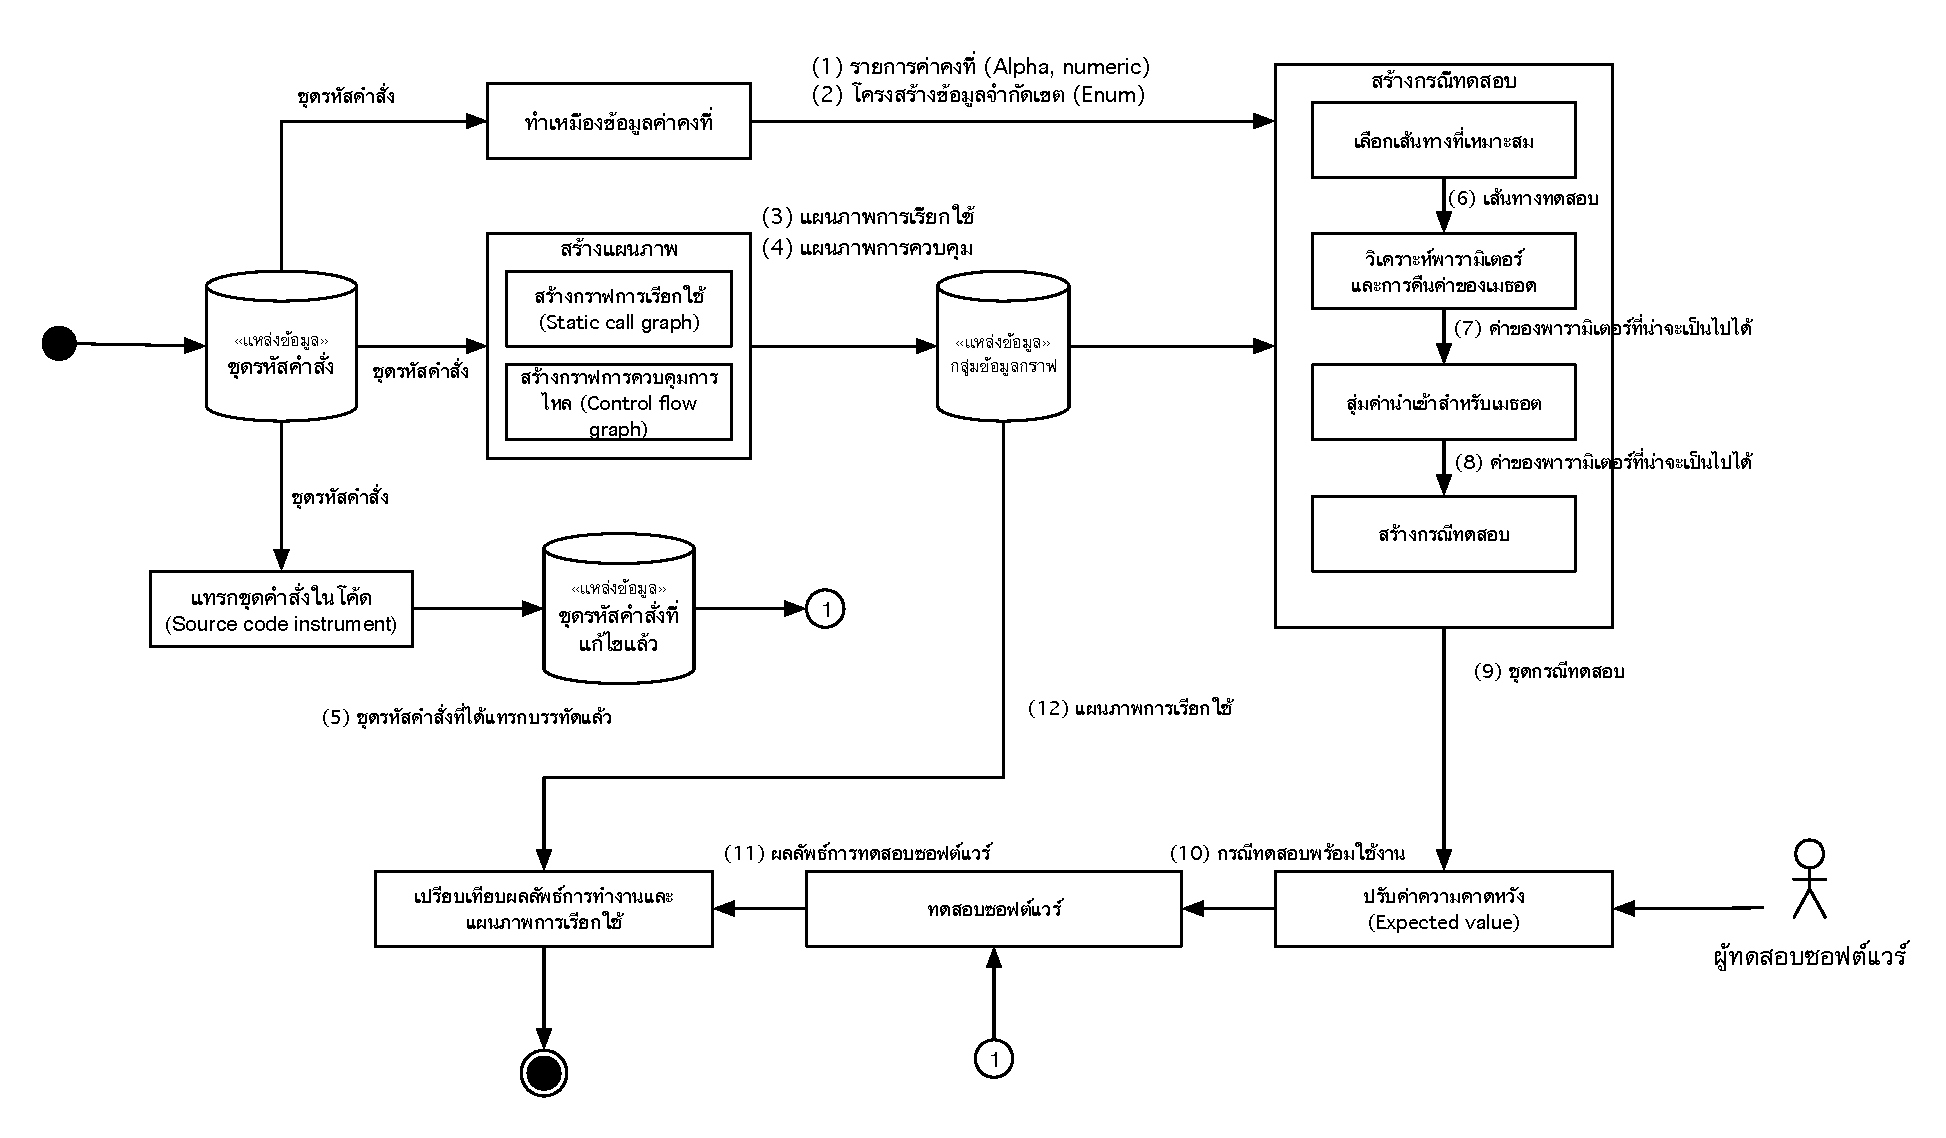
\includegraphics[width=\textwidth]{methodology-overview}
        \caption{ภาพรวมการดำเนินงานวิจัย}
        \label{fig:methodologyoverview}
    \end{figure}
\end{centering}

% - - - - - - - - - - - - - - - - - - - -
\subsection{การวิเคราะห์ข้อมูลเบื้องต้น}
\label{subs:introsection}

ในขั้นตอนนี้เริ่มต้นด้วยการนำเข้าข้อมูลแพคเกจและแหล่งข้อมูล{\sourcecode}ซึ่ง{\tester}ต้องการสร้างกรณีทดสอบไว้ในฐานข้อมูล 
เพื่อใช้เป็นข้อมูลในการวิเคราะห์ข้อมูล{\sourcecode} จากนั้นจึงทำสำเนา{\sourcecode}จาก{\Repository} ตามที่ผู้ใช้งานระบุเข้ามาเก็บไว้ภายในฐานข้อมูล  เพื่อใช้รวบรวม{\StaticInformation} 
โดยสนใจเพียงเฉพาะ{\class}ซึ่งบรรจุอยู่ภายใน\FirstTimeDefine{\Package}{\PackageEN} ตามที่ผู้ใช้งานระบุ 
โดยกำหนดให้เป็น {\bf \CUT} ทั้งนี้กระบวนการจะประกอบไปด้วย 3 ขั้นตอนด้วยกัน นั่นคือ
{\constantExtracting}, {\graphCreation} 
และ{\sourcecodeInstrumention} 
โดยมีแนวทางการดำเนินงานของแต่ละขั้นตอน ดังนี้

% - - - - - - - - - - - - - - - - - - - -
% - - - - - - - - - - - - - - - - - - - -
\subsubsection{\constantExtracting}
\label{sec:sub:sub:sourceCodeExtract}

ขั้นตอนนี้เป็นกระบวนการเพื่อกำหนดแนวทางการในการสร้างข้อมูลทดสอบสำหรับ{\TestPath}ที่เลือก โดยมีแนวทางการจัดเก็บค่าคงที่ที่ประกาศไว้
ภายใน{\sourcecode} โดยสนใจกลุ่มข้อมูล 2 กลุ่ม ได้แก่

\begin{enumerate}
    \item {\it ข้อมูลพื้นฐาน (Primitive data)} ซึ่งเป็นข้อมูลพื้นฐานที่ใช้งานภายใน{\class} ซึ่งในที่นี้จะสนใจข้อมูลพื้นฐาน 2 ประเภทได้แก่
        \begin{enumerate}
            \item {\bf ตัวอักษร} ซึ่งมีประเภทข้อมูลเป็น \code{String} ในภาษาจาวา
            \item {\bf ตัวเลข} ซึ่งมีประเภทข้อมูล ได้แก่ \code{byte, short, int, long, float} และ\,\code{double} ในภาษาจาวา
        \end{enumerate}
    \item {\it {\enum} (Enumeration)} ซึ่งมีประเภทข้อมูลเป็น \code{enum} ในภาษาจาวา
\end{enumerate}

ทั้งนี้จะไม่สนใจข้อมูลเชิงตรรกะ (มีชนิดข้อมูลเป็น \code{bool} ในภาษาจาวา) เนื่องจากว่าตัวเลือกที่เป็นไปได้นั้นมีเพียง 2 ตัวเลือกเท่านั้น
นอกจากนั้นจะยังไม่สนใจข้อมูลจำเพาะ ที่กำหนดขึ้นมาใช้งานเอง 
จาก{\sourcecode}ของ{\class} \code{SimpleBonusScore} และ\,\code{SimpleGrading} ดังที่แสดงใน 
\figref{fig:javaBonusScore} และ \ref{fig:javaGrading} ตามลำดับ ในการดำเนินการวิจัยครั้งนี้ 
จะจัดเก็บข้อมูลค่าคงที่ซึ่งอยู่ในบรรทัดที่ \code{6, 8, 9, 10, 11, 12, 15, 16, 17} และ \code{18} ของ{\class} \code{SimpleBonusScore}
ตลอดจนค่าคงที่ซึ่งอยู่ในบรรทัดที่ \code{4, 5, 6, 8, 9} และ \code{10} ของ{\class} \code{SimpleGrading} 
แล้วจึงนำมาจัดเก็บไว้ภายในฐานข้อมูลโดยแยกตาม{\class}ที่พบค่าคงที่เหล่านั้น เพื่อใช้ในขั้นตอน {\bf \testcaseGeneration} ต่อไป

หลังจากรวบรวม{\bf ค่าคงที่}จาก{\sourcecode}ได้เรียบร้อยแล้ว จะนำ{\bf ข้อมูลพื้นฐาน} และ{\bf {\enum}} ที่รวบรวมได้
จัดหมวดหมู่และบันทึกไว้ภายใน{\it ฐานข้อมูล}

% - - - - - - - - - - - - - - - - - - - -
% - - - - - - - - - - - - - - - - - - - -
\subsubsection{\graphCreation}
\label{sec:sub:sub:graphCreation}

กระบวนการสร้างกราฟนั้นจะรับข้อมูล{\sourcecode}จาก{\Repository}ร่วมกับข้อมูลแพคเกจที่{\tester}สนใจมาประกอบกัน 
เพื่อใช้สร้างกราฟ โดยแบ่งออกเป็น 2 กระบวนการย่อยด้วยกัน คือ การสร้าง{\scg} และการสร้าง{\cfg} โดยมีรายละเอียดดังต่อไปนี้

\begin{enumerate}
    \item {\bf สร้าง{\scg}} ขั้นตอนนี้จะอ่านข้อมูล{\CUT}ตามรายการไฟล์ใน{\Package}ที่ผู้ใช้งานสนใจ 
        แล้วจึงค้นหา{\callingStatement} เพื่อกำหนด{\callingMethod}และ{\calledMethod}ตามลำดับ 
        โดยเริ่มต้นจาก{\class}ที่พบ{\method}~\code{main}~เป็นลำดับแรกเพื่อหา{\Node}เริ่มต้นหรือ{\Node}หัว
        และ{\class}ปลายทางซึ่งปรากฎ~\calledMethod~เป็น{\Node}หาง 
        ดังนั้นหาก{\sourcecode}ของ{\SUT}ประกอบด้วยคลาส~\code{C_1,~C_2~C_3} ซึ่งแต่ละคลาสจะประกอบไปด้วย{\method}
        \code{\{m_{11},~m_{12}\}},~\code{\{m_{21},~m_{22},~m_{23}\}}, และ \code{\{m_{31},~m_{32}\}} ตามลำดับ
        ซึ่งปรากฎ{\callingStatement}ภายใน{\method}~\code{m_{11}}~เรียกไปยัง{\method}~\code{m_{21}},
        และ~\code{m_{22}} ซึ่งในขั้นตอนนี้จะรวมรวม{\callingStatement}ที่พบทั้งหมดในทุก ๆ {\class}ของ{\SUT}
        เพื่อสร้างเป็นกราฟดัง~\figref{fig:exampleSCG} โดยผลลัพธ์ที่ได้นั้นจะแบ่งเป็น 3 กลุ่ม ได้แก่
        \begin{enumerate}
            \item การเรียกใช้งานระหว่าง{\CUT}ด้วยกัน \label{ord:scgcut} 
            \item การเรียกใช้งานระหว่าง{\CUT}และ{\class}ภายในชุดพัฒนาของจาวา (Java SDK) \label{ord:scgjdk} 
            \item การเรียกใช้งานระหว่าง{\CUT}และชุดคำสั่งภายนอก (\code{3^{rd}} party library) \label{ord:scg3rd} 
        \end{enumerate}
        \-\hspace{1cm}ซึ่งในแนวทางการดำเนินงานนี้จะสนใจเฉพาะ{\scg}ของ{\CUT}เท่านั้น 
        ดังนั้นในขั้นตอนนี้ไม่สนใจกราฟที่เกิดจากการเรียกใช้ในข้อ 1.2 
        และ 1.3 ตลอดจนกราฟที่เกิดจากการสร้างวัตถุใหม่ เพื่อให้ได้{\scg}เฉพาะ{\CUT} ดังเช่น{\scg}โปรแกรมคํานวณเกรดนิสิต 
        ใน\figref{fig:scggrading}

    \item {\bf สร้าง{\cfg}} โดยจะอ่านข้อมูลของ{\CUT} ทีละ{\method} เพื่อนำมาสร้าง{\cfg}แสดงโครงสร้างภายใน{\method}
        หาก \code{G_{11}} แทน{\cfg}ของ{\method}~\code{m_{11}} และให้ \code{G_1~=~\{G_{11},~G_{12}\}} 
        เป็นเซตของ{\cfg}ของแต่ละ{\method}ของ{\class}~\code{C_1} จาก\figref{fig:exampleSCG} 
        จะเก็บข้อมูลของ{\CUT}เพื่อสร้าง \code{G_2}~และ~\code{G_3} ซึ่งเป็นเซตของ{\cfg}ของแต่ละ{\method}ของ{\class}
        \code{C_2} และ \code{C_2} ซึ่งข้อมูลที่ได้นี้จะจัดเก็บข้อมูลไว้ภายในฐานข้อมูลต่อไป
        ทั้งนี้ในขั้นตอนนี้จะสร้างเส้นทางที่เป็นไปได้ซึ่งสั้นที่สุดโดยเริ่มต้นจาก{\sourcenode}ไปยัง{\sinknode}ของแต่ละ{\method} 
        โดยจะต้องเป็นเส้นทางที่ผ่าน{\callingStatement}
\end{enumerate}

\begin{figure}
    \centering
    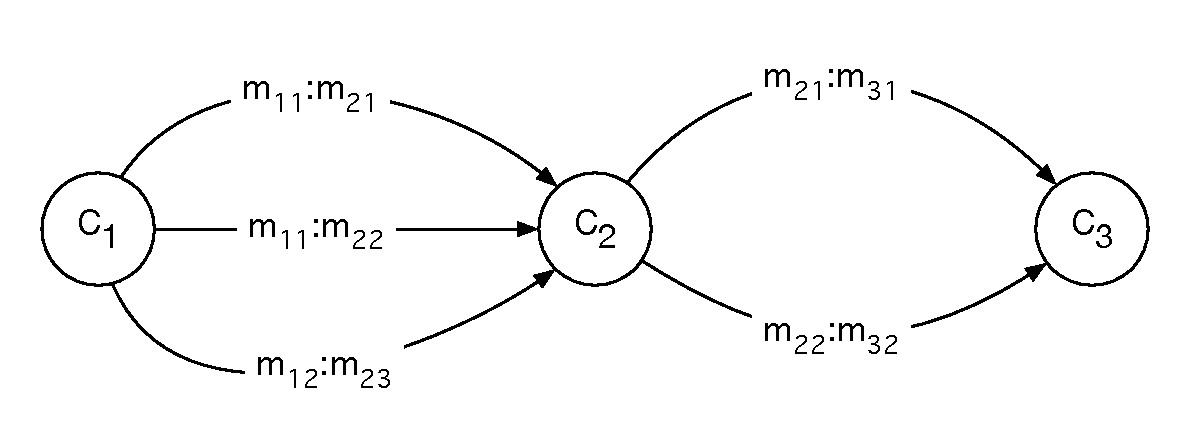
\includegraphics[width=.9\textwidth]{example-scg}
    \caption{ตัวอย่าง{\scg}สำหรับคลาส \code{C_1,~C_2,}~และ~\code{C_3}}
    \label{fig:exampleSCG}
\end{figure}

เมื่อสิ้นสุดกระบวนการจะนำข้อมูล{\bf {\scg}} และ{\bf {\cfg}} ที่ได้จัดเก็บลง {\it ฐานข้อมูล} เพื่อจัดเตรียมไว้สำหรับ 
{\bf ขั้นตอนการสร้างกรณีทดสอบ} และ{\bf เปรียบเทียบผลลัพธ์การดำเนินการ} ต่อไป

% - - - - - - - - - - - - - - - - - - - -
% - - - - - - - - - - - - - - - - - - - -
\subsubsection{\sourcecodeInstrumention}
\label{sec:sub:sub:srcInstrument}

เนื่องจากการทดสอบนี้จำเป็นต้องครอบคลุม{\Path}ระหว่าง{\CUT} ดังนั้นจำเป็นต้องแทรกชุดคำสั่งใน{\sourcecode}ในแต่ละขั้นตอนการทำงาน 
จากนั้นจึงนำ{\sourcecode}ที่ผ่านการแทรกชุดคำสั่งเรียบร้อยแล้วไปใช้ในกระบวนการทดสอบ 
แล้วจึงจัดเก็บผลลัพธ์ที่ได้ระหว่างขั้นตอนการทดสอบ แล้วจึงนำมาเปรียบเทียบกับ{\TestPath}ที่เลือกเพื่อหาความครอบคลุมของ{\scg}ถัดไป

เมื่อเสร็จสิ้นกระบวนการแทรกชุดคำสั่ง จะนำ{\sourcecode}ที่ได้จัดเก็บไว้ใน {\it ฐานข้อมูล} เพื่อจัดเตรียมไว้สำหรับนำไปทดสอบอีกครั้ง

% - - - - - - - - - - - - - - - - - - - -
\subsection{\testcaseGeneration}
\label{sec:sub:tcg}

การดำเนินงานวิจัยในครั้งนี้จะนำ {\bf ข้อมูลกราฟ} ซึ่งประกอบไปด้วย {\it {\scg}} ร่วมกับ{\it {\cfg}} ใช้เป็นข้อมูลเริ่มต้นเพื่อสร้าง{\TestPath}
ระหว่าง{\CUT} ให้ครอบคลุมความสัมพันธ์ระหว่าง{\class} ดังที่ปรากฎใน{\scg} 
สร้างกรณีทดสอบซึ่งพิจารณาจาก{\PredicateNode}ที่ปรากฎบน{\TestPath}ที่เลือก แล้วจึงนำข้อมูลทั้งหมดที่ได้สร้างเป็นชุดกรณีทดสอบ 
โดยมีภาพรวมการดำเนินงานดัง \figref{fig:testcaseGenerationActivity}

\begin{figure}[ht!]
    \centering
    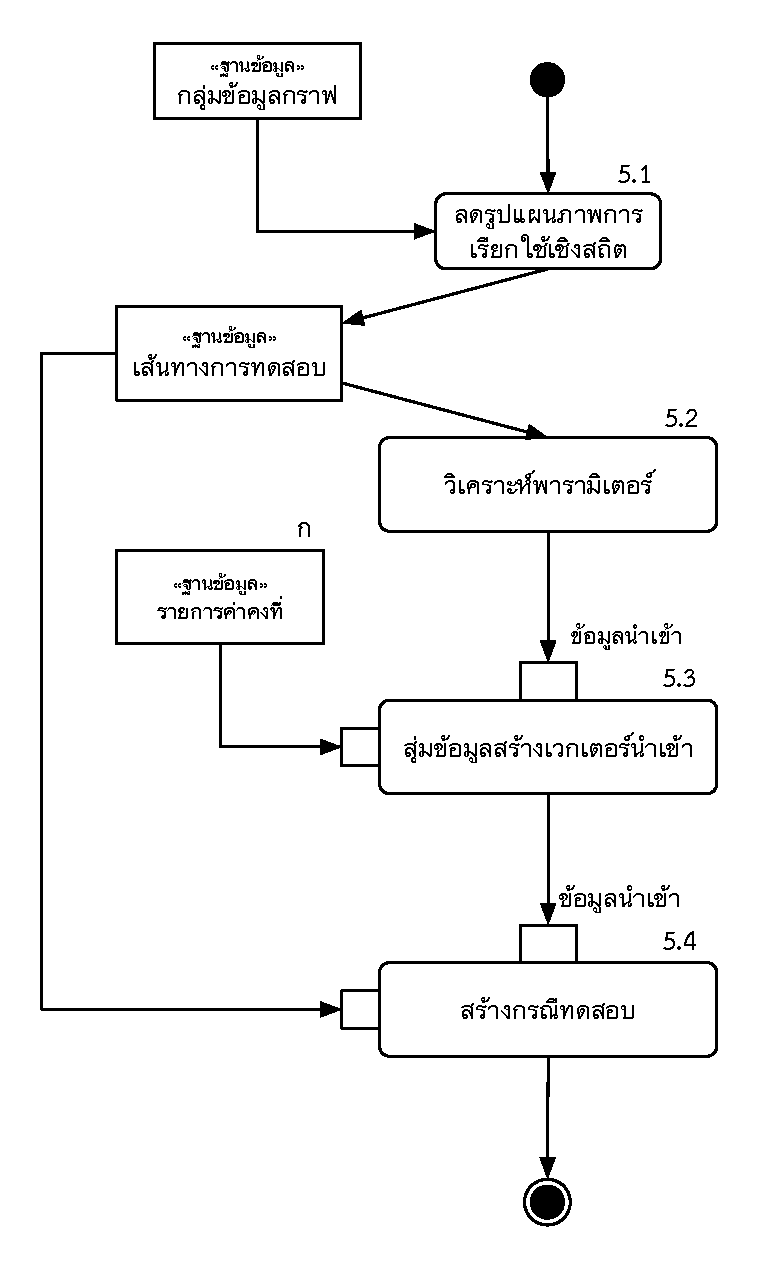
\includegraphics[width=0.45\textwidth]{methodology-activities-test-case-gen}
    \caption{ขั้นตอนการสร้างกรณีทดสอบ}
    \label{fig:testcaseGenerationActivity}
\end{figure}

% - - - - - - - - - - - - - - - - - - - -
% - - - - - - - - - - - - - - - - - - - -
\subsubsection{\testpathSelection}

ในขั้นตอนนี้จะพิจารณาจากข้อมูล{\it \scg} ร่วมกับ {\it \cfg} เพื่อเลือก{\TestPath}ที่ครอบคลุมความสัมพันธ์ระหว่าง{\class}ที่ปรากฎบน{\scg} 
เฉพาะระหว่าง{\CUT} ซึ่งจาก{\scg}ตัวอย่างใน\figref{fig:scggrading} จะได้{\TestPath} 2 {\Path} ด้วยกันคือ

\begin{figure}[ht!]
    \centering
    \begin{tikzpicture}[shorten >=1pt, node distance=5cm, auto,]
        \node(p1){\code{P_1:}};
        \node[right of=p1, xshift=-4.4cm](g1){\code{G}};
        \node[right of=g1](s1){\code{B}};
        \node[right of=s1](q1){\code{Q}};
        %
        \node[below of=p1,yshift=4cm](p2){\code{P_2:}};
        \node[right of=p2, xshift=-4.4cm](g2){\code{G}};
        \node[right of=g2](s2){\code{B}};
        \node[right of=s2](q2){\code{Q}};
        %
        % Path
        \path(g1) edge [] node {\code{grading:score}} (s1);
        \path(s1) edge [] node {\code{score:getQuizScore}} (q1);
        %
        \path(g2) edge [] node {\code{grading:score}} (s2);
        \path(s2) edge [] node {\code{score:getQuizSum}} (q2);
    \end{tikzpicture}
    \caption{{\TestPath}จาก{\scg}}
    \label{fig:testPathFromSCG}
\end{figure}

เพื่อให้ทราบถึง{\pathConditions}บน{\TestPath} จึงใช้{\cfg}ของ{\method} \code{grading} จาก{\class} \code{SimpleGrading}, 
{\method} \code{score} จาก{\class} \code{SimpleBonusScore} รวมทั้ง{\method} \code{getQuizeScore} และ \code{getQuizSum} จาก{\class} \code{SimpleQuiz}
รวมพิจารณา ดัง\figref{fig:callreferences}

\begin{figure}[h!]
    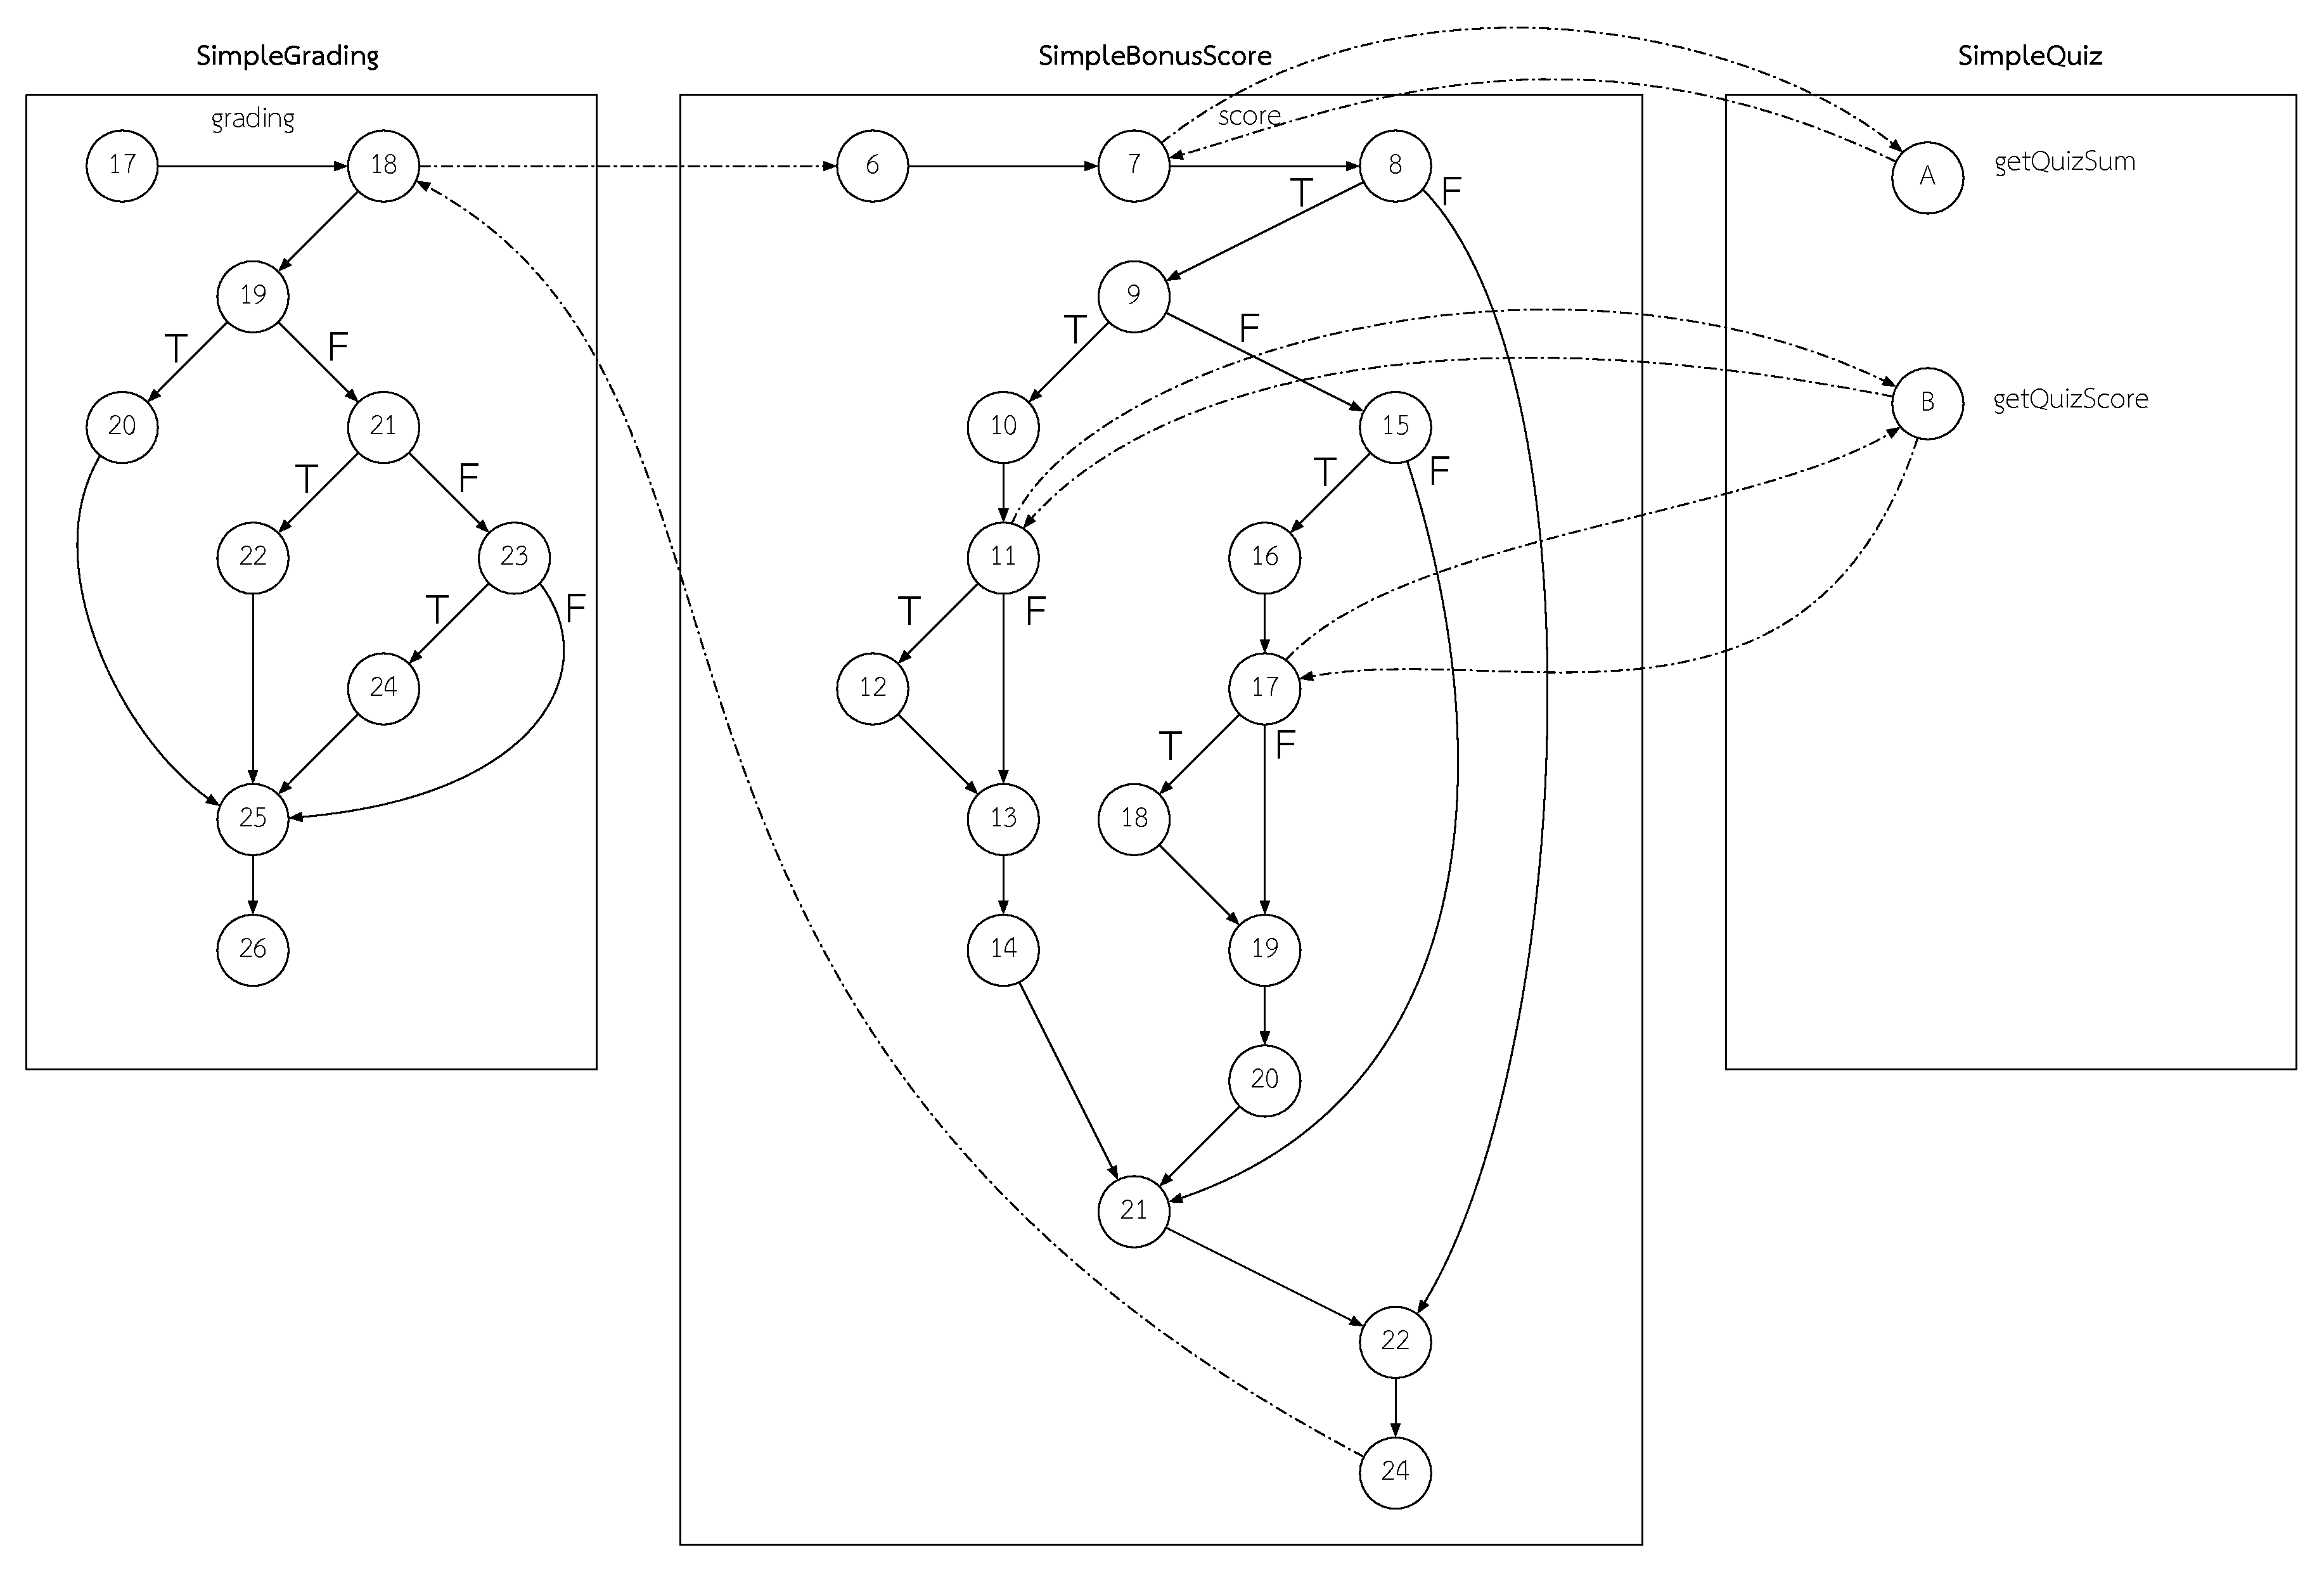
\includegraphics[width=\textwidth]{test-path-selection-call-reference}
    \caption{\mbox{โครงสร้างความสัมพันธ์ของ\class\,\code{SimpleGrading},\,\code{SimpleBonusScore} และ\,\code{SimpleQuiz}}}
    \label{fig:callreferences}
\end{figure}

\newpage
ซึ่งมีแนวทางการเลือก{\TestPath} ดังนี้
\begin{enumerate}
    \item เลือก{\TestPath}ที่สั้นที่สุดก่อนเสมอ
    \item เลือก{\TestPath}ที่พบ{\PredicateNode}น้อยที่สุดก่อนเสมอ
    \item เลือก{\TestPath}ไปยังทิศที่ทำให้{\PredicateNode}มีค่าความจริงเป็นจริงก่อนเสมอ
\end{enumerate}

เมื่อพิจารณาข้อมูลกราฟดัง \figref{fig:callreferences} จะได้{\TestPath} \code{P_1} ดัง\figref{fig:exampleTestPathP1}
\begin{figure}
    \centering
    \code{P_1: \underbrace{17-18}_{G}-\overbrace{6-7}^{B}-\underbrace{A}_{Q}-\overbrace{7-\overline{8}-22-24}^{B}-\underbrace{18-19-20-25-26}_{G}} 
    \caption{รายการของ{\Node}ที่ต้องพิจารณาของ{\TestPath} \code{P_1}}
    \label{fig:exampleTestPathP1}
\end{figure}

% - - - - - - - - - - - - - - - - - - - -
% - - - - - - - - - - - - - - - - - - - -
\subsubsection{การวิเคราะห์พารามิเตอร์และการคืนค่าของ{\method}}

แนวทางในขั้นตอนนี้จะนำ{\TestPath}ที่ได้คัดเลือกไว้ในขั้นตอนก่อนหน้านี้ (ซึ่งในที่นี้คือ \code{P_1} และ\code{P_2}) มาพิจารณาข้อมูลนำเข้า
และพารามิเตอร์ของแต่ละ{\method}ที่มีการเรียกผ่านกัน โดยจะเริ่มพิจารณาที่{\PredicateNode}ที่อยู่ในลำดับท้ายสุดของ{\TestPath}ก่อนเสมอ 
แล้วจึงนำเงื่อนไขการสร้างข้อมูลของทั้งเส้นทางมากำหนดกรอบสำหรับการสร้างข้อมูล 
ยกตัวอย่างเช่น \code{P_1} จะพบ{\PredicateNode}ทั้งสิ้น 2 {\Node} ด้วยกัน ได้แก่ {G: 19} และ \code{S: 8}
ซึ่งมีเงื่อนไขดังนี้

\begin{enumerate}
    \item[\code{G:19}] \code{student\_score < SCORE\_MINIMUM\_SATISFIED} \label{itm:studentscore}
    \item[\code{S:8}]  \code{bonus\_score > 0} \label{itm:studentid}
\end{enumerate}

โดยในขั้นตอนนี้จะนำค่าคงที่ที่เก็บไว้ในขั้นตอน {\bf \constantExtracting}} มาแทนในตัวแปร \code{SCORE\_MINIMUM\_SATISFIED} 
(\code{SCORE\_MINIMUM\_SATISFIED} มีค่าเท่ากับ \code{80}) แล้วจึงพิจารณาข้อมูลทดสอบจากเงื่อนไขข้างต้น
เพื่อสร้างกรณีทดสอบและข้อมูลทดสอบที่เข้าทดสอบ{\TestPath}ตามที่เลือกได้ โดยที่ข้อมูลที่สร้างขึ้นนั้นจะต้องทำให้เงื่อนไข 
\code{G:19} เป็นจริง (\code{True}) และเงื่อนไข \code{S:8} เป็นเท็จ (\code{False})

% - - - - - - - - - - - - - - - - - - - -
% - - - - - - - - - - - - - - - - - - - -
\subsubsection{\randomTestData}
\label{sec:sub:randomTestData}

สำหรับแนวทางการดำเนินงานในขั้นตอนนี้จะรับเงื่อนไขการสร้าง{\testData}จากกระบวนการก่อนหน้าเพื่อนำมาสร้างข้อมูลทดสอบ 
เพื่อให้กรณีทดสอบสามารถทดสอบ{\TestPath}ตามที่เลือกได้ ตามวิธีการที่กำหนด \cite{XING201491, Ma2016, Heaton2000} 
หากมีพารามิเตอร์ที่ไม่ปรากฎใน{\TestPath}เป็นข้อมูลนำเข้า จะใช้วิธีการสุ่ม{\testData}โดยอาศัยค่าคงที่ประกอบการพิจารณา

เมื่อพิจารณาข้อมูล\FirstTimeDefine{\MethodSignature}{\MethodSignatureEN} ของ{\method} \code{score} 
ของ{\class} \code{SimpleGrading} พบว่า{\method}นี้ต้องการพารามิเตอร์ทั้งหมด 3 ค่า ด้วยกัน คือ \code{student\_id:String}, 
\code{student\_score:int} และ~\code{bonus\_score:int} 
แต่จากตัวแปรที่พบใน{\PredicateNode}นั้นจะมีเพียง \code{student\_score} และ~\code{bonus\_score} 
จึงใช้เงื่อนไขที่พบนั้นเป็นแนวทางการสร้าง{\testData}{\TestPath} คงเหลือตัวแปร \code{student\_id} จึงใช้การสุ่มข้อมูลเพื่อสร้าง{\testData}
โดยพิจารณาจากค่าคงที่ที่มีประเภทข้อมูลแบบเดียวกัน ซึ่งจัดเก็บ{\sourcecode}จากกระบวนการก่อนหน้า 
ซึ่งกำหนดให้ข้อมูลทดสอบที่สร้างขึ้นได้ในกระบวนการนี้มีรายการดัง~\tabref{tab:GRTRandom}

\begin{table}[ht!]
    \centering
    \caption{ตัวอย่าง{\randomTestData}ที่ได้}
    \label{tab:GRTRandom}
    \begin{tabularx}{\textwidth}{|*3{>{\centering\arraybackslash}X|}@{}}
        \hline
        \rowcolor{LightGray}
        ตัวแปร                    & ประเภทข้อมูล   & ค่าที่สุ่มได้          \\ \hline
        \code{student\_score}    & {\it int}    & {\bf 75}         \\ \hline
        \code{bonus\_score}      & {\it int}    & {\bf 0}         \\ \hline
        \code{student\_id}       & {\it String} & {\bf "IUUUSISS"} \\ \hline
    \end{tabularx}
\end{table}

% - - - - - - - - - - - - - - - - - - - -
% - - - - - - - - - - - - - - - - - - - -
\subsubsection{\testcaseGeneration}
\label{sec:sub:sub:tcGen}

ในขั้นตอนนี้จะนำข้อมูลนำเข้าที่สร้างจากกระบวนการก่อนหน้ามาสร้างกรณีทดสอบสำหรับภาษาจาวา โดยใส่{\expectedOutput} (บรรทัดที่ 7) 
จะเกิดจากการสุ่มโดยอิงตามประเภทข้อมูลที่{\method}นั้นคืนค่า ดังตัวอย่างของกรณีทดสอบภายใน {\it \testSuite} ดัง\figref{fig:junitGradingTest}

\begin{figure}[ht!]
    \lstset{basicstyle=\small,style=thesiscodestyle}
    \lstinputlisting[language=Java]{methodology/SimpleGradingTest.java}
    \caption{กรณีทดสอบที่สร้างขึ้นจากข้อมูลทดสอบ}
    \label{fig:junitGradingTest}
\end{figure}

% - - - - - - - - - - - - - - - - - - - -
\subsection{\expectedOutputAdjustment}
\label{sec:sub:expectedOutputAdj}

ในขั้นตอนนี้\tester จะทำหน้าที่ปรับค่า\FirstTimeDefine{\expectedOutput}{\expectedOutputEN}
แนวทางการดำเนินงานในขั้นตอนนี้จะเป็นการปรับค่าข้อมูลที่อยู่ภายในกรณีทดสอบที่ได้รับโดยนักทดสอบซอฟต์แวร์ 
เพื่อให้กรณีทดสอบนั้นสอดคล้องกับการทำงานที่ควรจะเป็นของโปรแกรมมากที่สุด ยกตัวอย่างเช่นกรณีทดสอบที่ได้จากขั้นตอนที่ \ref{sec:sub:tcg} 
ดัง\figref{fig:junitGradingTest} 
เมื่อได้ปรับค่าคาดหวังจากนักทดสอบซอฟต์แวร์แล้วจะได้เป็นดัง{\figref{fig:junitGradingTestRefined}
ซึ่งในที่นี้นักทดสอบซอฟต์แวร์ได้ปรับค่าในบรรทัดที่ 5 โดยเปลี่ยนจาก \code{"IUUUSISS"} ให้เป็นค่า \code{"5873000021"} 
และบรรทัดที่ 7 คือค่า \code{"lorem"} เป็นค่า \code{"U"} จะได้ตัวอย่างของ {\it กรณีทดสอบพร้อมใช้งาน} 
ดัง\figref{fig:junitGradingTestRefined}

\begin{figure}[ht!]
    \lstset{style=thesiscodestyle}
    \lstinputlisting{methodology/SimpleGradingTest-Refined.java}
    \caption{กรณีทดสอบที่สร้างขึ้นจากข้อมูลทดสอบที่ปรับค่าจากนักทดสอบซอฟต์แวร์แล้ว}
    \label{fig:junitGradingTestRefined}
\end{figure}

\subsection{\executeSoftwareTesting}
\label{sec:sub:executeSoftwareTesting}

แนวทางการดำเนินงานในขั้นตอนนี้จะรับ {\it ชุดกรณีทดสอบ} 
ทดสอบร่วมกับ{\sourcecode}ที่{\it \sourcecodeInstrumention}จาก{\it ฐานข้อมูล} 
และรวบรวมข้อมูลที่เกิดจากชุดคำสั่งที่แทรกไว้ ซึ่งปรากฎขึ้นระหว่างการทดสอบเข้าไว้ด้วยกันเป็น {\it ผลลัพธ์การทดสอบซอฟต์แวร์} 
เพื่อใช้ตรวจสอบให้แน่ใจว่ากรณีทดสอบนั้นสามารถทดสอบ{\TestPath}ที่เลือกได้ 

\subsection{\testResultCompare}
ในขั้นตอนนี้จะรับ {\it ผลลัพธ์การทดสอบซอฟต์แวร์} มาสร้างเส้นทางการทดสอบเทียบกับ{\TestPath}ที่ได้เลือกไว้ก่อนหน้านี้ 
เพื่อให้แน่ใจได้ว่าชุดทดสอบที่สร้างขึ้นนั้นครอบคลุม{\scg}ตาม{\TestPath}ที่กำหนดไว้ และแสดงผลลัพธ์กลับให้{\tester}ทราบ


    \section{วัตถุประสงค์ของงานวิจัย}
\label{sec:objective}
    ศึกษา ออกแบบ และพัฒนาเครื่องมือแนวทางการสร้างการกรณีทดสอบจาก{\TestPath}ที่ได้จาก{\scg}สำหรับภาษาจาวา\label{obj:designandresearch}


    \section{ขอบเขตงานวิจัย}
\label{sec:limitation}

\begin{enumerate}
    \label{enu:limitation}
    \item สร้างกรณีทดสอบที่ครอบคลุม{\TestPath}ระหว่าง{\CUT} \label{enu:lim:tc}
    \item รองรับการเรียกใช้งานกันของ{\CUT}บน{\TestPath}สูงสุด 3 {\class} \label{enu:lim:3linkingclass}
    \item รองรับ{\method}ภายใน{\CUT}สูงสุดไม่เกิน 5 {\method}ต่อ{\class} \label{enu:lim:5methods}
    % \item รองรับ{\class}ภาษาจาวาขนาดความยาวไม่เกิน 200 บรรทัดต่อ{\class} \label{enu:lim:200loc} 
        % http://softwareengineering.stackexchange.com/questions/66523/how-many-lines-per-class-is-too-many-in-java
    % \item รองรับ{\TestPath}ที่ปรากฎ{\PredicateNode}ตลอดทั้ง{\Path}ไม่เกิน 20 {\Node}  \label{enu:lim:20predicate}
    \item ข้อมูล{\scg}ที่สร้างขึ้นนั้นจะสนใจเฉพาะความสัมพันธ์ระหว่างคลาสที่อยู่ภายใน{\Package}จาวา (Java package) ตามที่ผู้ใช้ระบุ 
        โดยยกเว้นชุดพัฒนามาตรฐานของภาษาจาวาและชุดคำสั่งภายนอก \label{enu:lim:scg}
    \item รองรับข้อมูลนำเข้าประเภทตัวอักษร (มีชนิดข้อมูลเป็น \code{String} ในภาษาจาวา) ตัวเลข 
        (มีชนิดข้อมูลเป็น \code{byte, short, int, long, float} และ \code{double} ในภาษาจาวา) และ{\enum} 
        (มีชนิดข้อมูลเป็น \code{enum} ในภาษาจาวา) ยังไม่รองรับประเภทข้อมูลเฉพาะที่สร้างขึ้นเอง \label{enu:lim:datatype}
    \item รองรับโปรแกรมประยุกต์ที่พัฒนาขึ้นเพื่อใช้งานบนเครื่องคอมพิวเตอร์ส่วนบุคคล และ{\sourcecode}พัฒนาขึ้นด้วยภาษาจาวา  \label{enu:lim:datatype}
        % โดยไม่รวมถึงโปรแกรมประยุกต์ประเภทเว็บแอปพลิเคชัน
    \item ครอบคลุมโปรแกรมที่ทำงานเป็นลำดับ (Sequential) ไม่ครอบคลุมการทำงานของโปรแกรมที่ทำงานเป็นภาวะพร้อมกัน (Parallel) \label{enu:lim:seq}
    \item รองรับเฉพาะโปรแกรมที่มีจำนวนของไซโคลเมทิกภายในคลาสรวมกันน้อยกว่าหรือเท่ากับ 15
    \item รองรับการสร้างกรณีทดสอบที่สอดคล้องตามรูปแบบของชุดพัฒนา JUnit
    % \item รองรับการดำเนินงานแบบวงวน (Loop) 1 รอบ \label{enu:lim:loop}
    \item ไม่รองรับการเรียกใช้ฟังก์ชันเวียนเกิด (Recursion)
\end{enumerate}


    \section{ขั้นตอนการดำเนินงาน}

\begin{enumerate}
    \item ศึกษางานวิจัยที่เกี่ยวข้อง
    \item ศึกษาวิธีการสร้าง{\scg}ในภาษาจาวา
    \item ศึกษาวิธีการสร้างข้อมูลทดสอบแบบสุ่มซึ่งสอดคล้องกับ{\PredicateNode}บน{\TestPath}
    \item กำหนดขอบเขตและแนวทางการวิจัย
    \item ดำเนินการวิจัย
    \begin{enumerate}
        \item รวบรวมข้อมูลทดสอบ
        \item พัฒนาเครื่องมือเพื่อวิเคราะห์{\scg}
        \item พัฒนาเครื่องมือสร้างกรณีทดสอบและข้อมูลนำเข้าที่สอดคล้องกับ{\TestPath}ที่เลือก จาก{\scg}ร่วมกับ{\cfg}
        \item ทดสอบและปรับปรุงผลการทำงานของเครื่องมือ
        \item สรุปผลการดำเนินงานและข้อเสนอแนะ
    \end{enumerate}
    \item จัดทำรายงานวิทยานิพนธ์
\end{enumerate}


    \section{ประโยชน์ที่คาดว่าจะได้รับ}

\begin{enumerate}
    \item แนวทางการสร้างกรณีทดสอบจาก{\scg}ที่สร้างขึ้น
    \item แนวทางการสร้างข้อมูลทดสอบที่สอดคล้องกับ{\TestPath}ที่เลือก
    \item เครื่องมือที่สร้างสามารถกรณีทดสอบจาก{\scg} และข้อมูลนำเข้าที่สอดคล้องกับ{\TestPath}
\end{enumerate}


    \clearpage
    % -------------------- 
    % References section
    % -------------------- 
    \bibliographystyle{acm}
    \bibliography{references}
    % --------------------

\end{document}

